\documentclass{disser}

\usepackage{caption}
\usepackage{xcolor}
\usepackage{float}
\usepackage{listings}
\usepackage{graphicx}
\usepackage{scrhack}

\hypersetup{
  pdfauthor={Burlakov V.S.},
  pdftitle={Research on the use of generative neural network models in the development of a dialogue agent creation system},
  pdfsubject={Vladimir Burlakov's Bachelor Thesis},
  pdfkeywords = {machine learning, natural language processing, generative AI, artificial intellegence, game development, T5}
}

\onehalfspacing

\definecolor{mygreen}{rgb}{0,0.6,0}
\definecolor{mygray}{rgb}{0.5,0.5,0.5}
\definecolor{mymauve}{rgb}{0.58,0,0.82}
\lstloadlanguages{Python}
\lstset{
  language=Python,
  keywordstyle={\bfseries \color{blue}},
  captionpos=b,
  basicstyle=\footnotesize,
  breaklines=true,
  breakatwhitespace=true,
  extendedchars=true,
  backgroundcolor=\color{white},
  commentstyle=\color{mygreen},
  escapeinside={\%*}{*)},
  stringstyle=\color{mymauve},
  numbers=left,
  numberstyle=\tiny\color{gray},
  tabsize=4,  % adjust to your preference
}

\graphicspath{ {./figures/} }

% Параметры названия для иллюстраций (Рисунок 1 - <название>)
\DeclareCaptionLabelFormat{PictureCaptionFormat}{Рисунок {#2}}
\captionsetup[figure] {
  labelformat=PictureCaptionFormat,
  skip=0pt,
  format=hang,
  justification=raggedright,
  labelsep=endash
}

% Параметры названия для таблиц (Таблица 1 - <название>)
\DeclareCaptionLabelFormat{TableCaptionFormat}{Таблица {#2}}
\captionsetup[table] {
  labelformat=TableCaptionFormat,
  skip=0pt,
  format=hang,
  justification=raggedright,
  singlelinecheck=off,
  labelsep=endash
}

\DeclareCaptionLabelFormat{ListingCaptionFormat}{Листинг {#2}}
\captionsetup[lstinputlisting] {
  labelformat=ListingCaptionFormat,
  skip=0pt,
  format=hang,
  justification=raggedright,
  labelsep=endash
}

\usetikzlibrary{matrix,chains,positioning,decorations.pathreplacing,arrows,arrows.meta}


\begin{document}

% 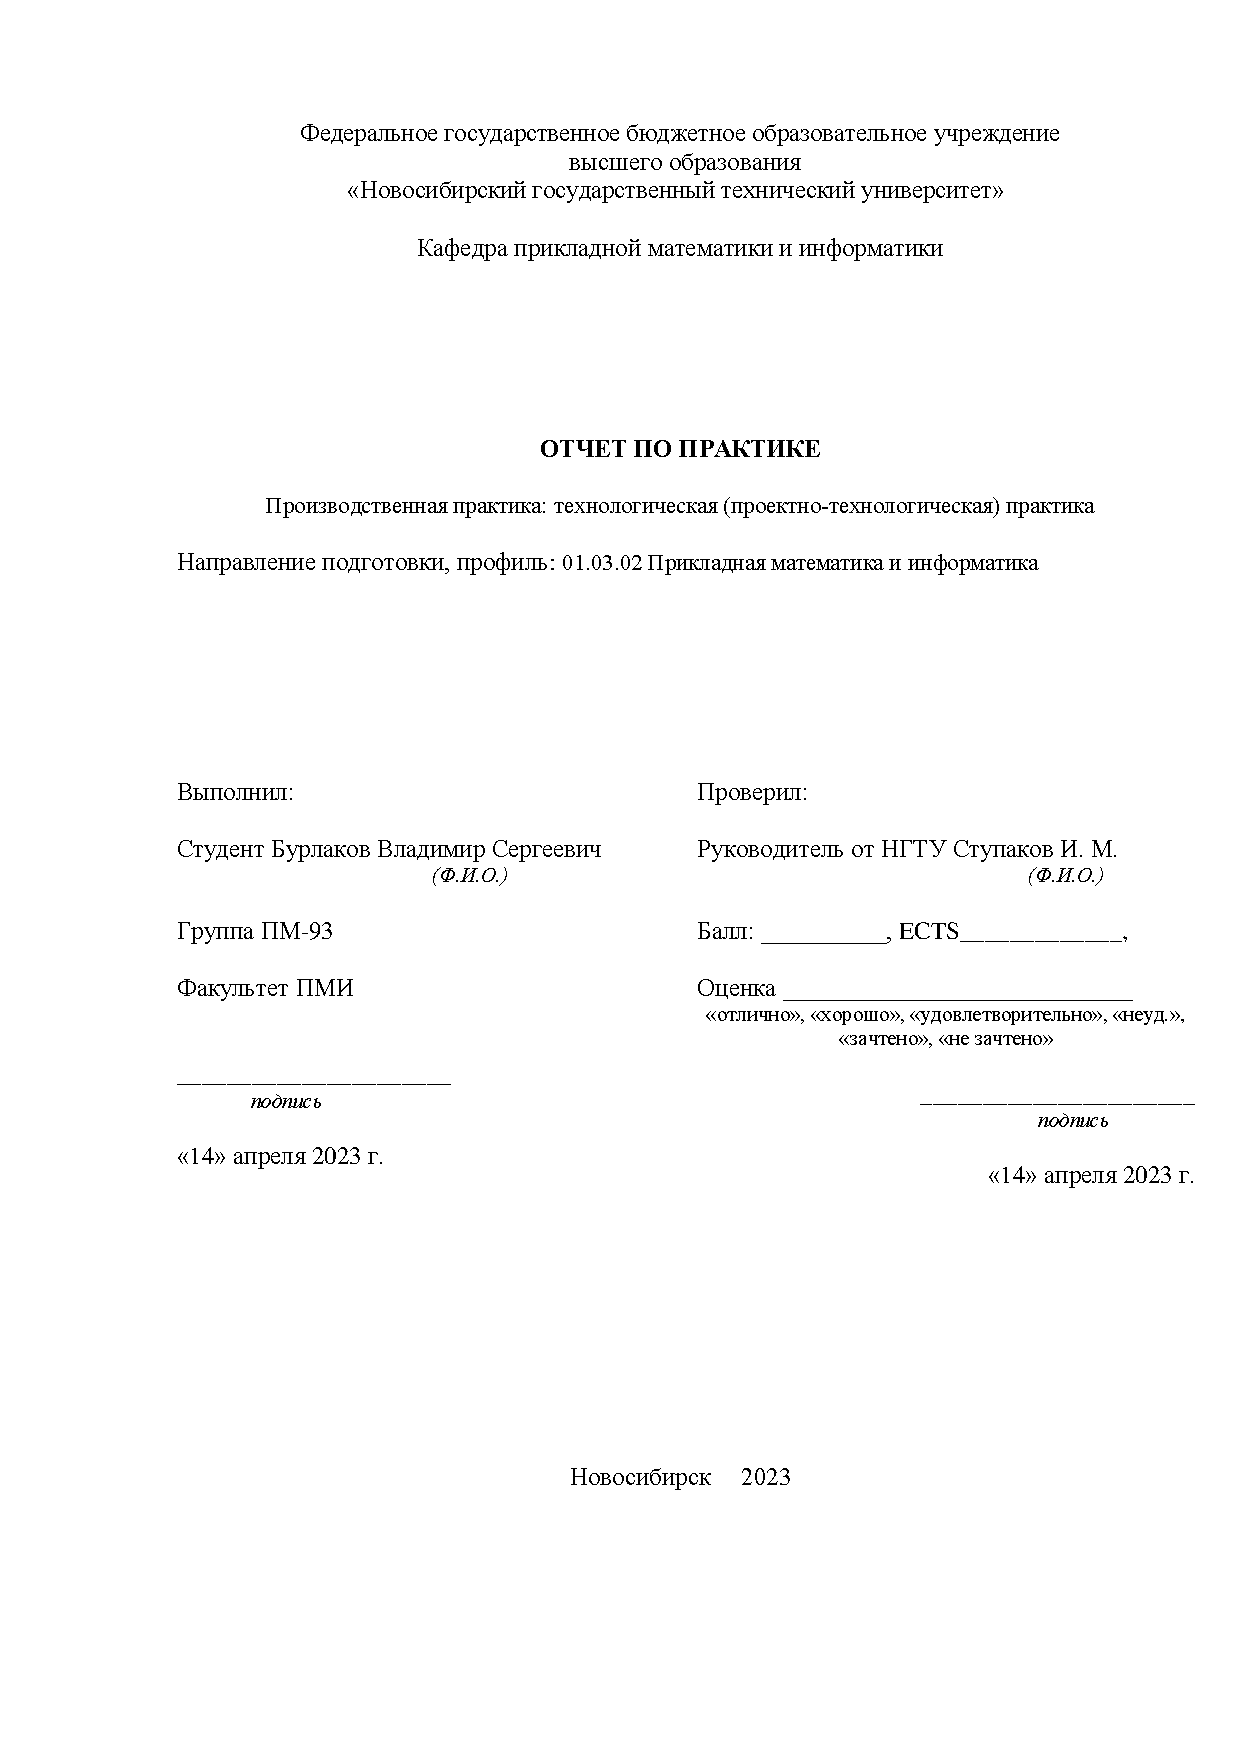
\includepdf{assets/title.pdf} % Титульный лист

\tableofcontents % Оглавление
\thispagestyle{empty}

\addchap{ВВЕДЕНИЕ}
% FROM FIRST PRACTICE
% В современных условиях растущей автоматизации взаимодействия человека с компьютером, создание эффективных диалоговых систем остается одним из важных направлений развития искусственного интеллекта. Такие технологии могут помочь во многих индустриях, в том числе игровой индустрии. Новейшие технологии, использующие глубокое обучение, позволяют создавать диалоговые модели, которые способны эффективно обрабатывать естественный язык и предоставлять пользователю качественные ответы на запросы. Для эффективного обучения диалоговых моделей необходимо обладать качественным набором данных, содержащим диалоги между участниками. В данной работе было решено расширить концепцию диалогового датасета путем включения описания личности участников разговора. Это имеет большое значение при использовании в игровой индустрии.В данном отчете рассматривается процесс создания и анализа датасета DNDD (Dungeon \& Dragons Dialogues) для обучения диалоговой модели, основанный на сборе и предобработке данных из различных источников.

Разработка диалоговых моделей является активно развивающейся областью машинного обучения. Использование таких моделей имеет широкий спектр применений, включая чат-ботов, системы FAQ, и различные другие системы, где взаимодействие с пользователем через естественный язык играет важную роль. В игровой индустрии диалоговые модели имеют особое значение, поскольку они способны создавать реалистичные и интерактивные диалоги с неигровыми персонажами, улучшая игровой опыт. Качественные диалоговые модели способны улучшить игровой опыт, создавая более привлекательные и погружающие виртуальные миры.

Целью данной работы является создание эффективной диалоговой модели, способную генерировать качественные ответы на основе образа неигрового персонажа и контекста диалога, обеспечивая более реалистичные и интерактивные диалоги с неигровыми персонажами, на основе датасета DNDD (Dungeon \& Dragons Dialogues), специально созданного для данного исследования. В данной работе рассматриваются подготовка датасета для обучения модели, формулирование задачи для моделирования, поиск оптимальной модели и параметров, необходимых для успешного и эффективного обучения. % Введение

\chapter{ПОДГОТОВКА ДАТАСЕТА DNDD ДЛЯ ОБУЧЕНИЯ МОДЕЛЕЙ}
%	\input{disser_tex/state-of-the-art} % Вставить куда-нить!
После фазы сбора диалоговых данных и генерации параметров неигровых персонажей, включающих в себя идентификаторы, характеристики, мировозрение, мотивацию и слабости, следующим логическим этапом становится подготовка собранных данных к процессу обучения модели. Этот процесс включает в себя конкатенацию данных в строковом формате.

\section{ЭМУЛЯЦИЯ ДИАЛОГОВЫХ ВЗАИМОДЕЙСТВИЙ}

Особое внимание следует уделить диалоговым взаимодействиям между неигровым персонажем и игроком. В контексте датасета, где хранятся полные версии диалогов, эмуляция процесса общения игрока с неигровым персонажем требует разбиения истории диалога на подмножества. В этом случае диалог представляет собой серию ходов между игроком и неигровым персонажем, и основной задачей модели является продолжение данного диалога, т.е. совершение следующего хода в диалоге.

При таком подходе модель обучается на основе итеративного процесса диалога, что способствует приближению к более реалистичному моделированию процесса диалога. Это позволяет на каждом этапе оптимизировать процесс обучения для достижения максимально эффективного результата.

\section{СТРУКТУРИРОВАНИЕ ВХОДНЫХ ДАННЫХ ДЛЯ ОБУЧЕНИЯ}

Для оптимизации процесса обучения, входные последовательности, а именно описание неигрового персонажа, история диалогов с игроком, последняя реплика игрока и реплика, которую должна сгенерировать модель, были разделены на сегменты, каждый из которых был помечен соответствующим образом. Такой подход к структурированию входных данных для модели позволяет ясно разделять различные компоненты входных данных, что облегчает задачу модели и способствует более эффективному обучению.

Для обозначения начала диалога используется уникальный идентификатор <<EMPTY>>, который функционирует как сигнал о том, что диалог только что был инициирован. В силу специфики датасета DNDD, полученного из игр, где неигровые персонажи всегда начинают диалог первыми, было определено, что первая реплика игрока служит активацией диалога, и обозначена она идентификатором <<START DIALOGUE>>. В ходе последующего диалога реплики участников регистрируются в истории диалога с пометками <<Player: >> и <<NPC: >>, в зависимости от того, кто в данный момент выступает в роли говорящего.

\section{ОПТИМИЗАЦИЯ ДАННЫХ ПОД ПОТРЕБИТЕЛЬСКОЕ ОБОРУДОВАНИЕ}

Учитывая ограниченные вычислительные ресурсы потребительского уровня, включая оперативную память объемом 32 гигабайта и графическую карту NVIDIA GeForce RTX 3090 Ti с 24 гигабайтами памяти, было необходимо ввести определенные ограничения на обрабатываемую историю диалогов. При превышении диалогом лимита в 1024 токенов, для обеспечения управляемости данных самые старые записи в диалоге подлежали удалению. Это позволяло оптимизировать использование доступных вычислительных ресурсов и обеспечивать стабильный процесс обучения моделей. 

Также было ограничено максимальное количество диалогов, которых может иметь игрок с одним неигровым персонажем. Это позволяет иметь меньшее, но более разнообразное количество данных.

Итоговые данные выглядят следующим образом.
Входная последовательность:
\texttt{\\Below is the definition of in-game NPC.\\
    NPC Name: Digby\\
    Alignment: Neutral\\
    Description: A burly, bearded man with a thick accent and a penchant for trapping.\\
    Personality traits: Digby is a bit of a glutton, and often overindulges in food and drink.\\
    Flaws: Digby is motivated by the prospect of making a profit from his trapping.\\
    Motivation: Digby is a gruff, no-nonsense man who is quick to anger and slow to trust. He is a hard worker and is not afraid to get his hands dirty. He is also a bit of a glutton, and often overindulges in food and drink.\\
    Dialogue history:\\
    Player: START DIALOGUE\\
    NPC: *burp* Think I had too much to drink last night. Heh! What am I sayin'?! There's no such thing, says my brothers. Hey, who are you, anyway?\\\\
    Player query: Who are you?\\
    Respond to player's query based on defined NPC:\\}

Ожидаемый ответ: \texttt{I'm Digby. I'm a trapper 'round these parts. Me and my brothers catch all sorts of varmints, skin 'em, and sell 'em. Course, it's hard lately now that Emmerich is pokin' 'round.}

Детальная реализация обработки датасета c документацией доступна в приложении \ref{app:code}.

\chapter{ОБУЧЕНИЕ МОДЕЛИ}
\section{ПОИСК ОПТИМАЛЬНОЙ МОДЕЛИ}

Генеративные модели обычно имеют большой размер, что создает сложности при исследовании таких моделей. Поэтому важным фактором при выборе модели является соотношение размера и качества. В настоящее время одним из самых сложных датасетов является MMLU \cite{bib1}, который проверяет знания моделей, полученных во время предварительного обучения, на различных задачах. Этот датасет включает задачи с разной степенью сложности, от простых до профессиональных. На данный момент наиболее оптимальной моделью на этом бенчмарке является Flan-T5-XL \cite{bib2} с 3 миллиардами параметров, имея результат $52.4\%$. Еще одной моделью, которая может составить ей конкуренцию, является LLAMA-13B \cite{bib3} c результатом $46.9\%$, но ее большой размер делает процесс обучения значительно более затратным по сравнению с Flan-T5-XL.

Flan-T5 является моделью семейства T5 \cite{bib4}, добавляющая в дообучающую выборку большое инструкций, что позволило значительно улучшить качество модели на новых задачах.

\section{ПОИСК ОПТИМАЛЬНЫХ ГИПЕРПАРАМЕТРОВ ДЛЯ МОДЕЛИ}
\subsection{ПОСТАНОВКА ЗАДАЧИ}

Из гиперпараметров, значетельно влияющих на процесс обучения модели, было выделено три группы:
\begin{enumerate}
  \item Планировщики скорости обучения:
        \begin{itemize}
          \item константный;
          \item константный с прогревом;
          \item линейный;
          \item косинусный;
          \item косинусный с перезагрузками;
          \item полиномиальный;
          \item обратный квадратный корень.
        \end{itemize}
  \item Cкорость обучения $\in \{1 \times 10^{-4}, 2 \times 10^{-4}, \ldots, 9 \times 10^{-4}, 1 \times 10^{-3}\}$.
\end{enumerate}

Оценка качества генерации моделей явялется сложной задачей и малоисследованной. В данной работе помимо значений функции ошибки на валидационных данных используются метрики Exact Match и MAUVE, позволяющие сравнивать параметры между собой. Модель обучалась с различными гиперпараметрами в группе, пока остальные параметры фиксировались.

Метрика Exact Match показывает, какой процент фраз при генерации совпал с ожидаемыми, а MAUVE подсчитывает то, насколько совпало распределенияе вероятностей сгенерированных фраз с распределением вероятностей ожидаемых фраз.

\subsection{АНАЛИЗ РЕЗУЛЬТАТОВ ЭКСПЕРИМЕНТОВ С ГИПЕРПАРАМЕТРАМИ}

При стартовой скорости обучения равной $1 \times 10^{-3}$ на ограниченном наборе данных были произведены эксперименты по поиску оптимального планировщика скорости обучения. В процессе экспериментов отмечается, что планировщик с обратным квадратным корнем не представлен на графиках, так как ни один из запусков эксперимента с использованием этого планировщика не был успешно завершен.

В ходе экспериментов большинство планировщиков не оказало заметного влияния на скорость обучения и метрики. Среди рассмотренных вариантов планировщиков, в среднем наилучшие результаты продемонстрировал константный планировщик. Наименее эффективным, но успешно завершившим процесс обучения, оказался линейный планировщик. Отмечается, что линейный планировщик характеризуется низким начальным значением функции ошибки на тренировочных и показывает наихудшие конечные значения на метрике MAUVE, что иллюстрируется на рисунках \ref{lr-s-train-loss} и \ref{lr-s-mauve}. График изменения скорости обучения представлен на рисунке \ref{lr-s-lr}. Ход экспериментов можно наблюдать на рисунках \ref{lr-s-train-loss}, \ref{lr-s-eval-loss}, \ref{lr-s-em}, \ref{lr-s-mauve}

% LR SCHEDULER
\begin{figure}[!ht]
  \centering
  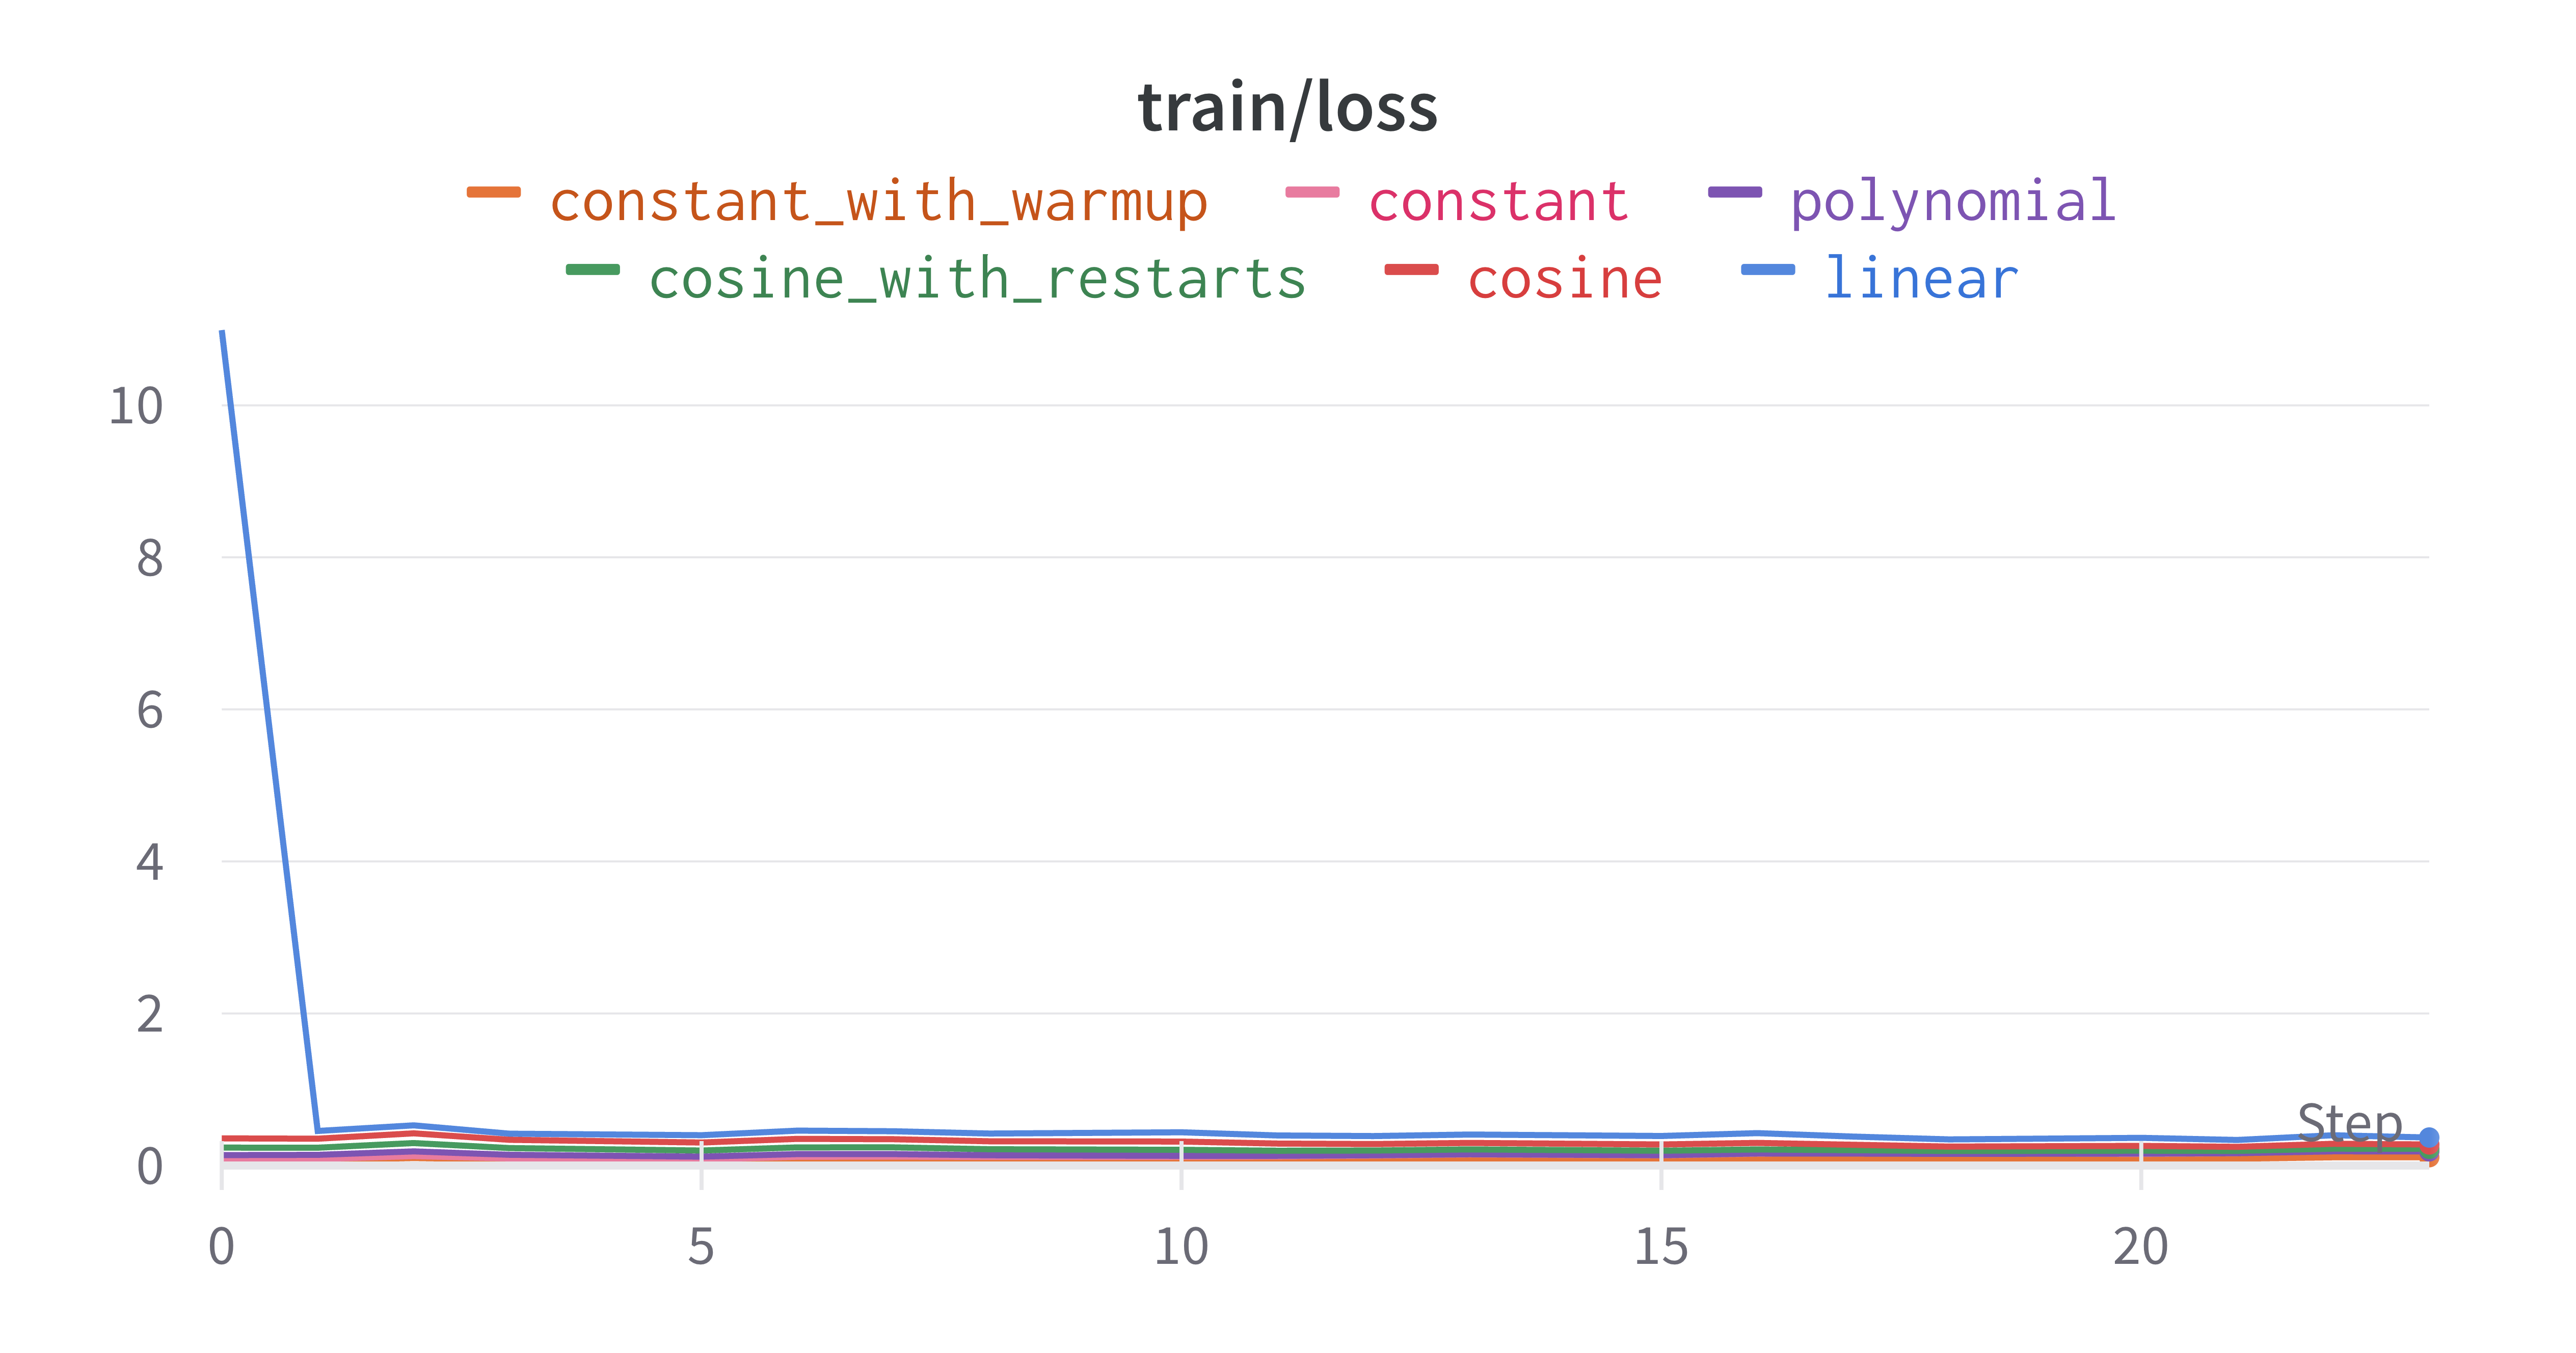
\includegraphics[width=.6\textwidth]{lr-s-train-loss}
  \caption{Значение функции ошибки на тренировочных данных}
  \label{lr-s-train-loss}
\end{figure}

\begin{figure}[!ht]
  \centering
  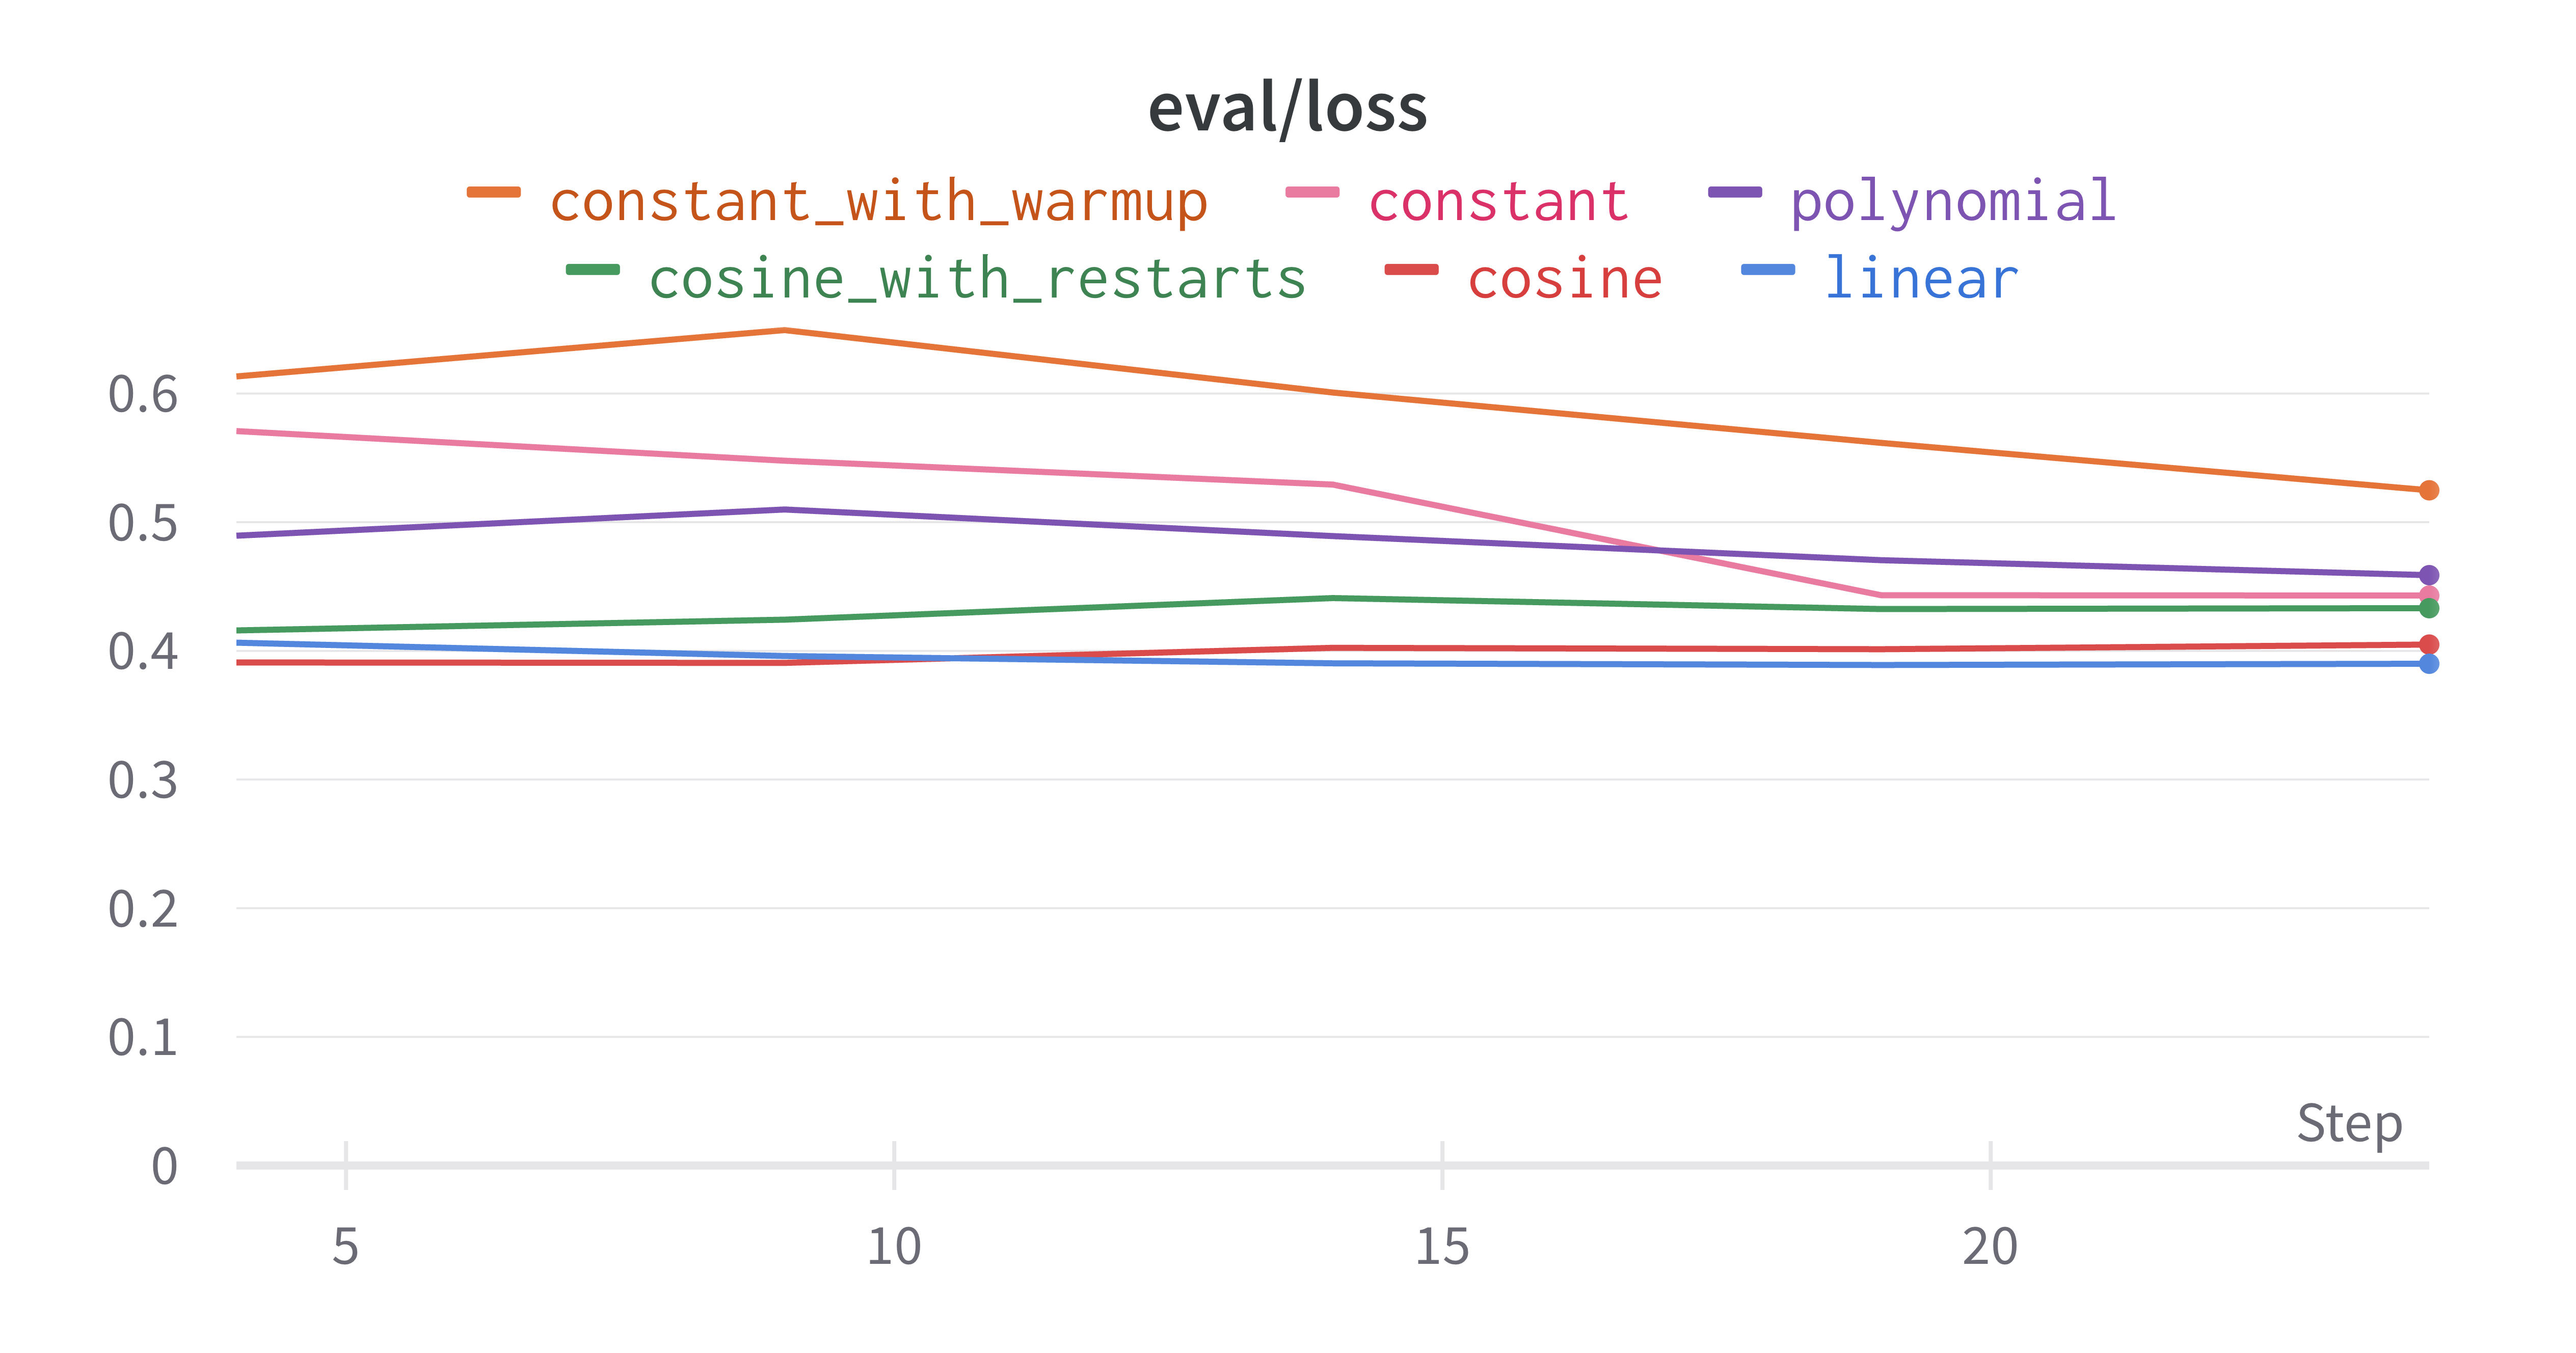
\includegraphics[width=.6\textwidth]{lr-s-eval-loss}
  \caption{Значение функции ошибки на валидационных данных}
  \label{lr-s-eval-loss}
\end{figure}

\begin{figure}[!ht]
  \centering
  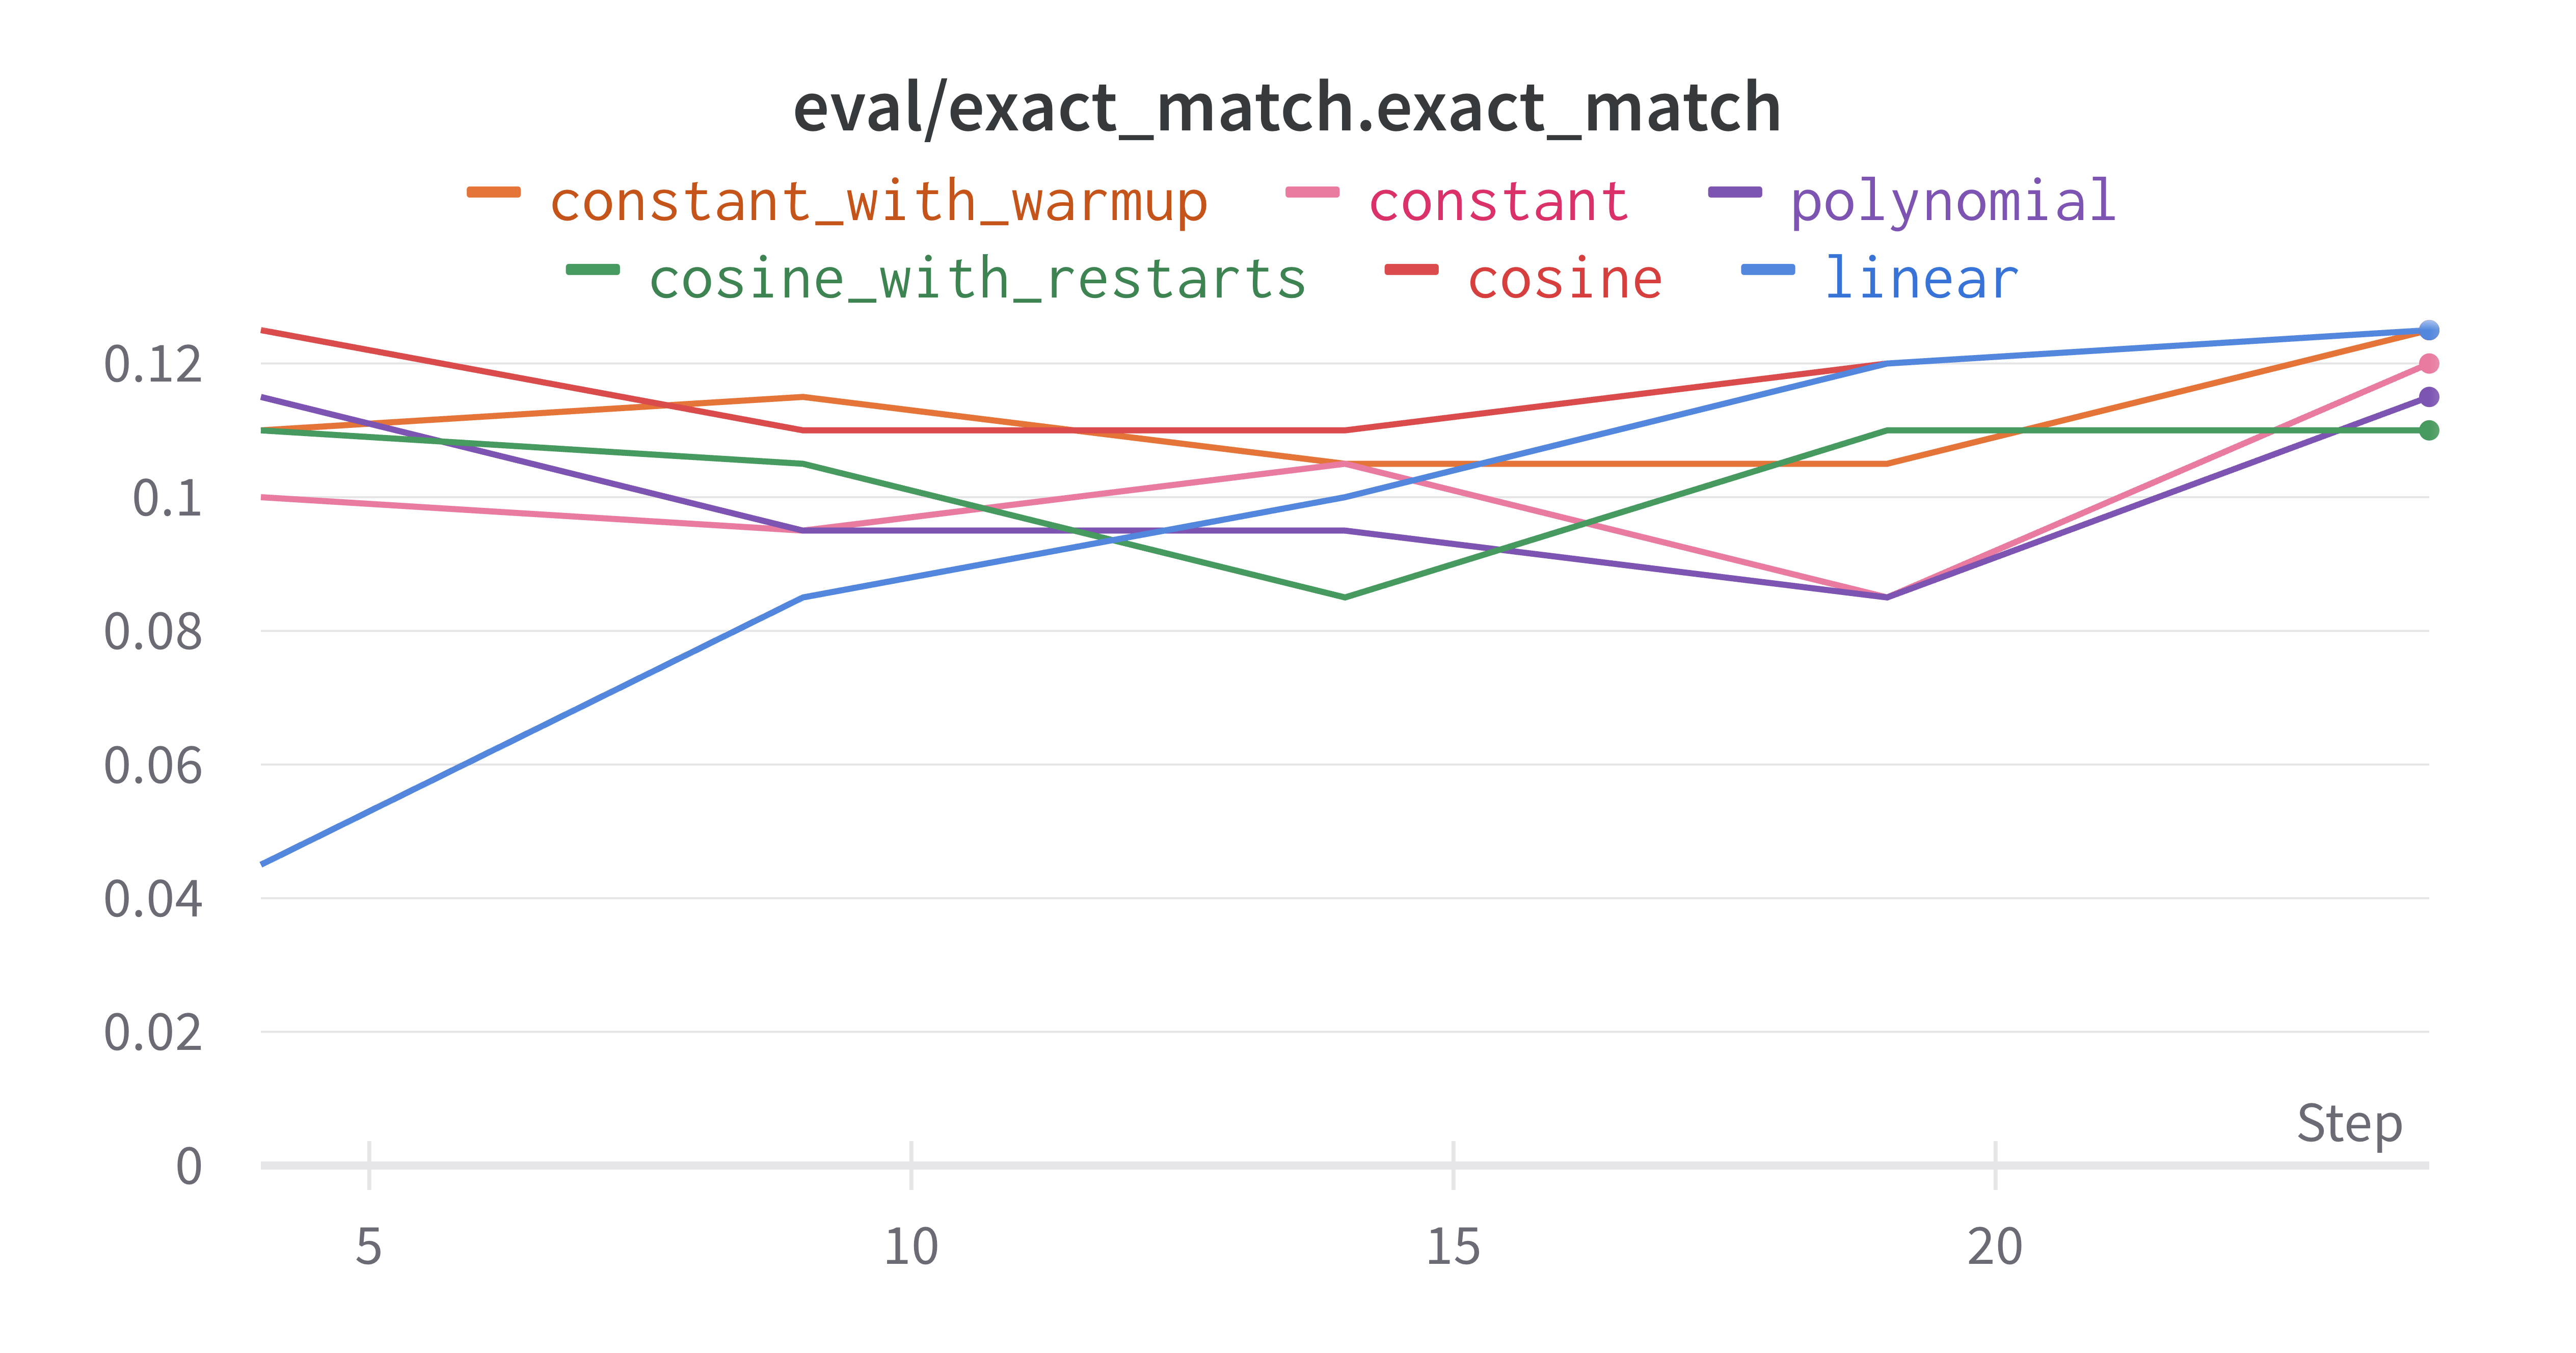
\includegraphics[width=.6\textwidth]{lr-s-em}
  \caption{Значение метрики Exact Match на валидационных данных}
  \label{lr-s-em}
\end{figure}

\begin{figure}[!ht]
  \centering
  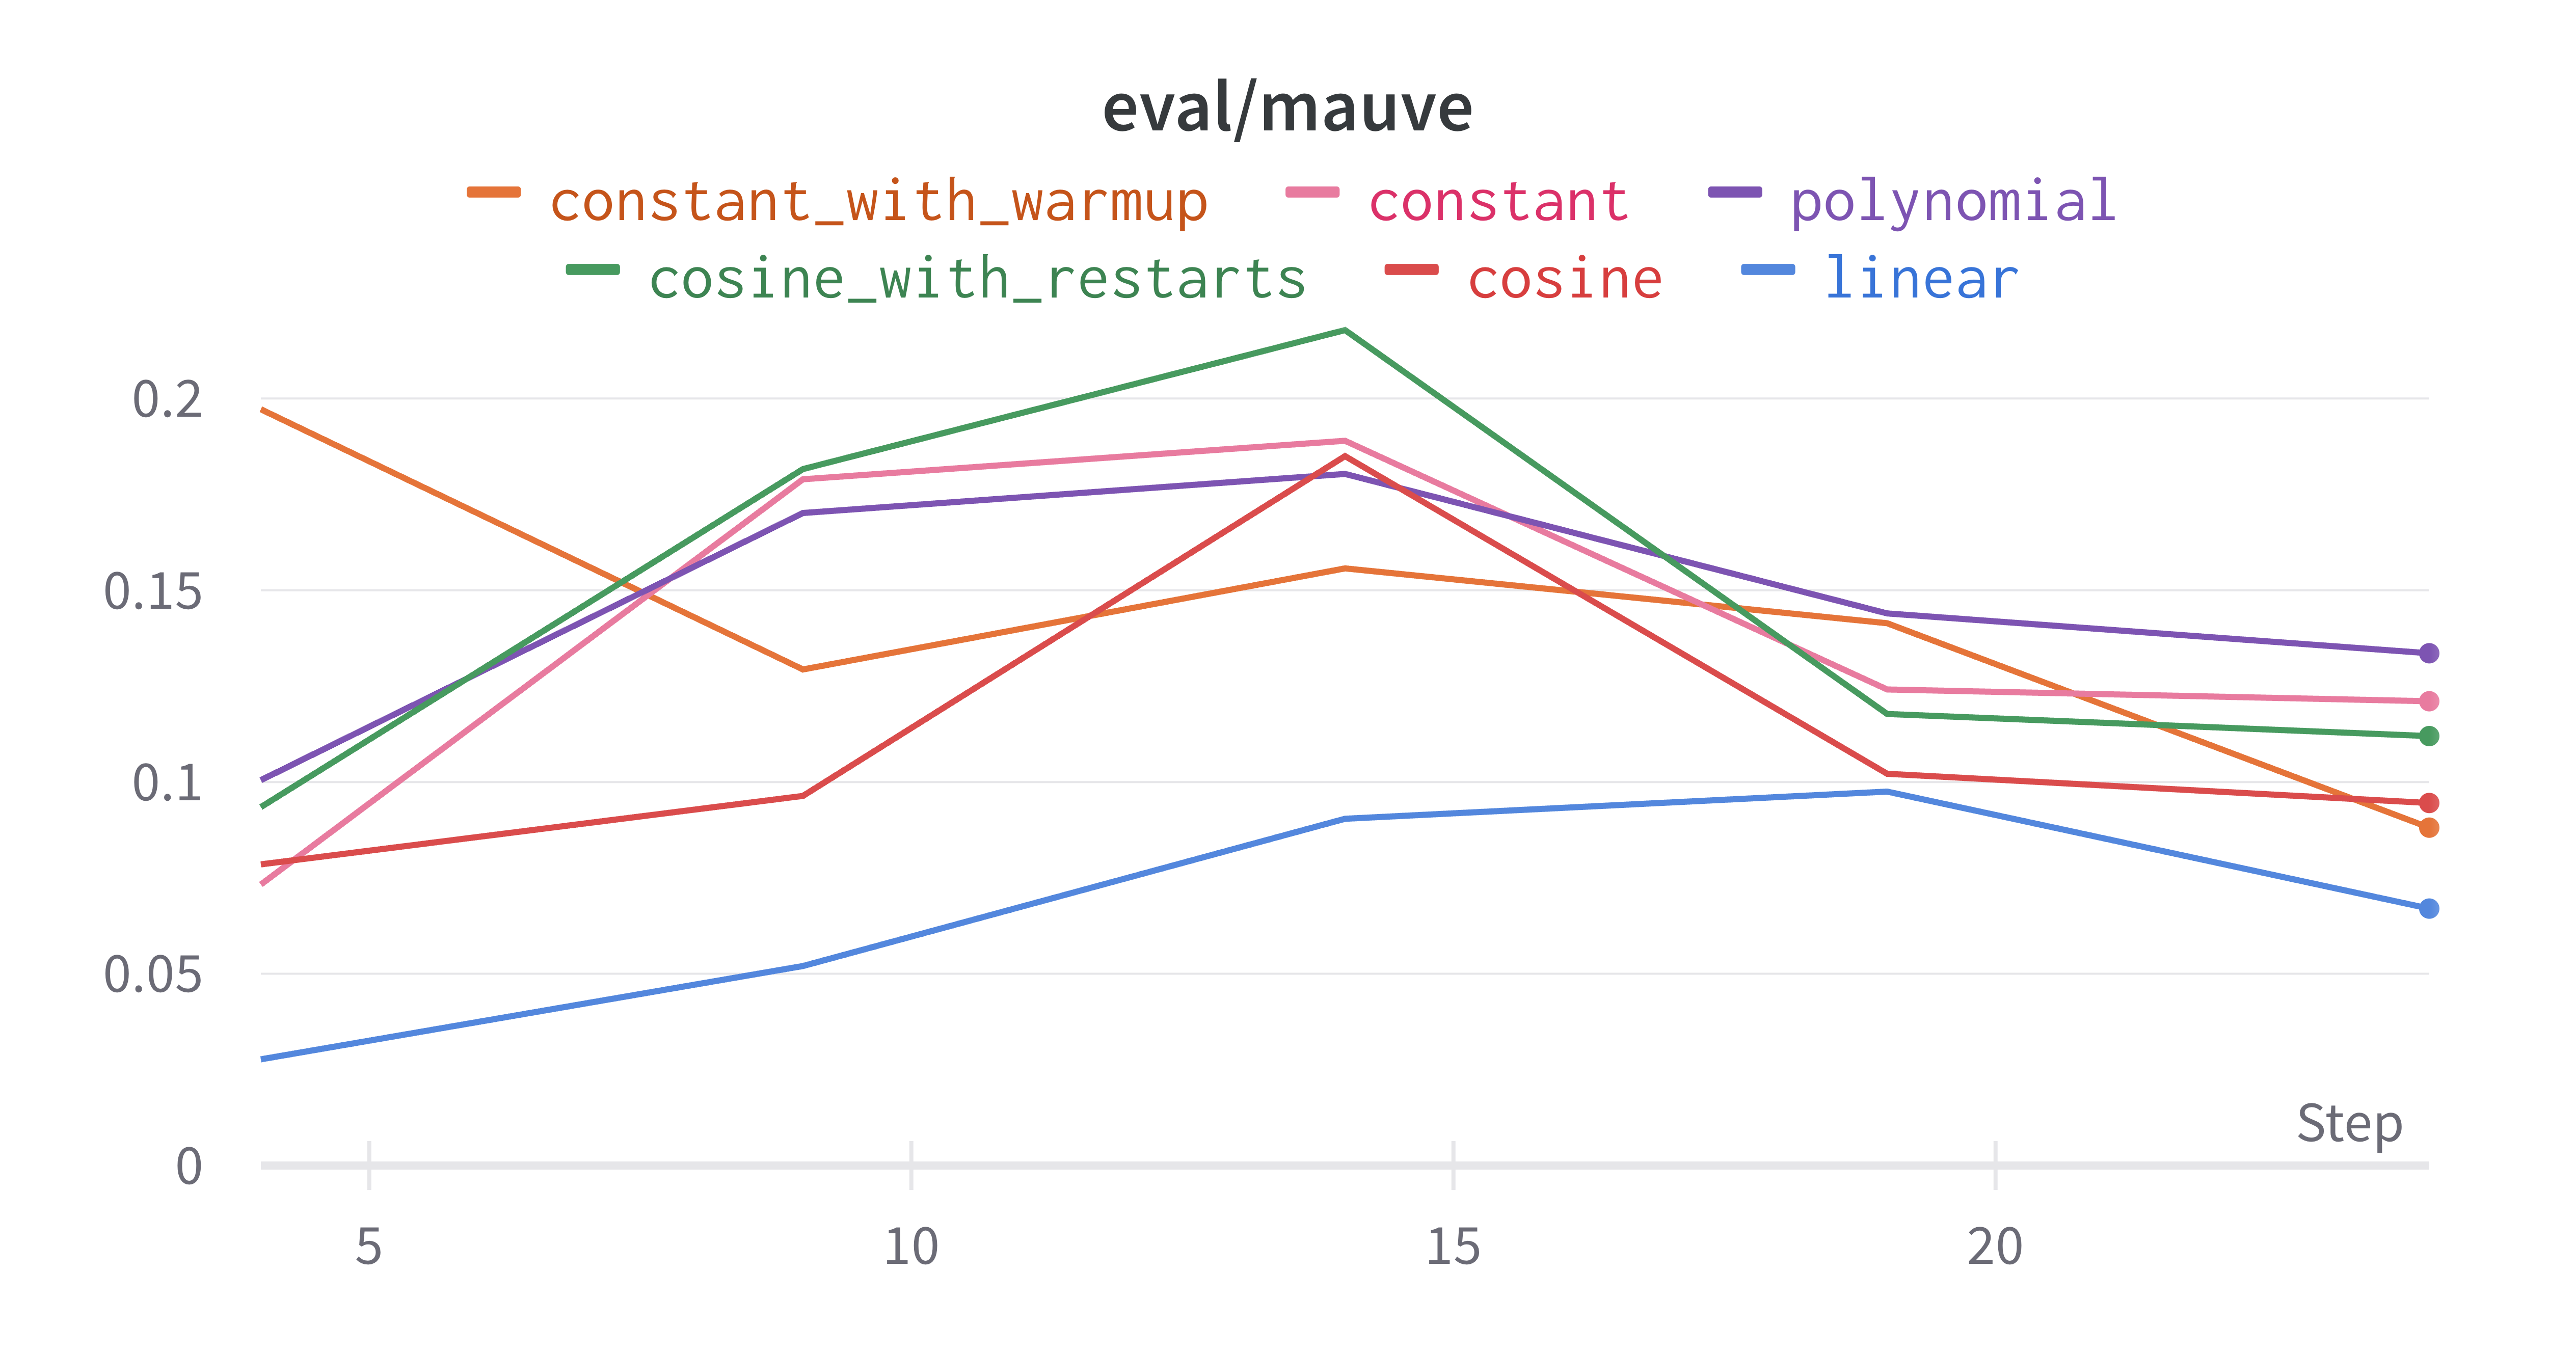
\includegraphics[width=.6\textwidth]{lr-s-mauve}
  \caption{Значение метрики MAUVE на валидационных данных}
  \label{lr-s-mauve}
\end{figure}

\begin{figure}[!ht]
  \centering
  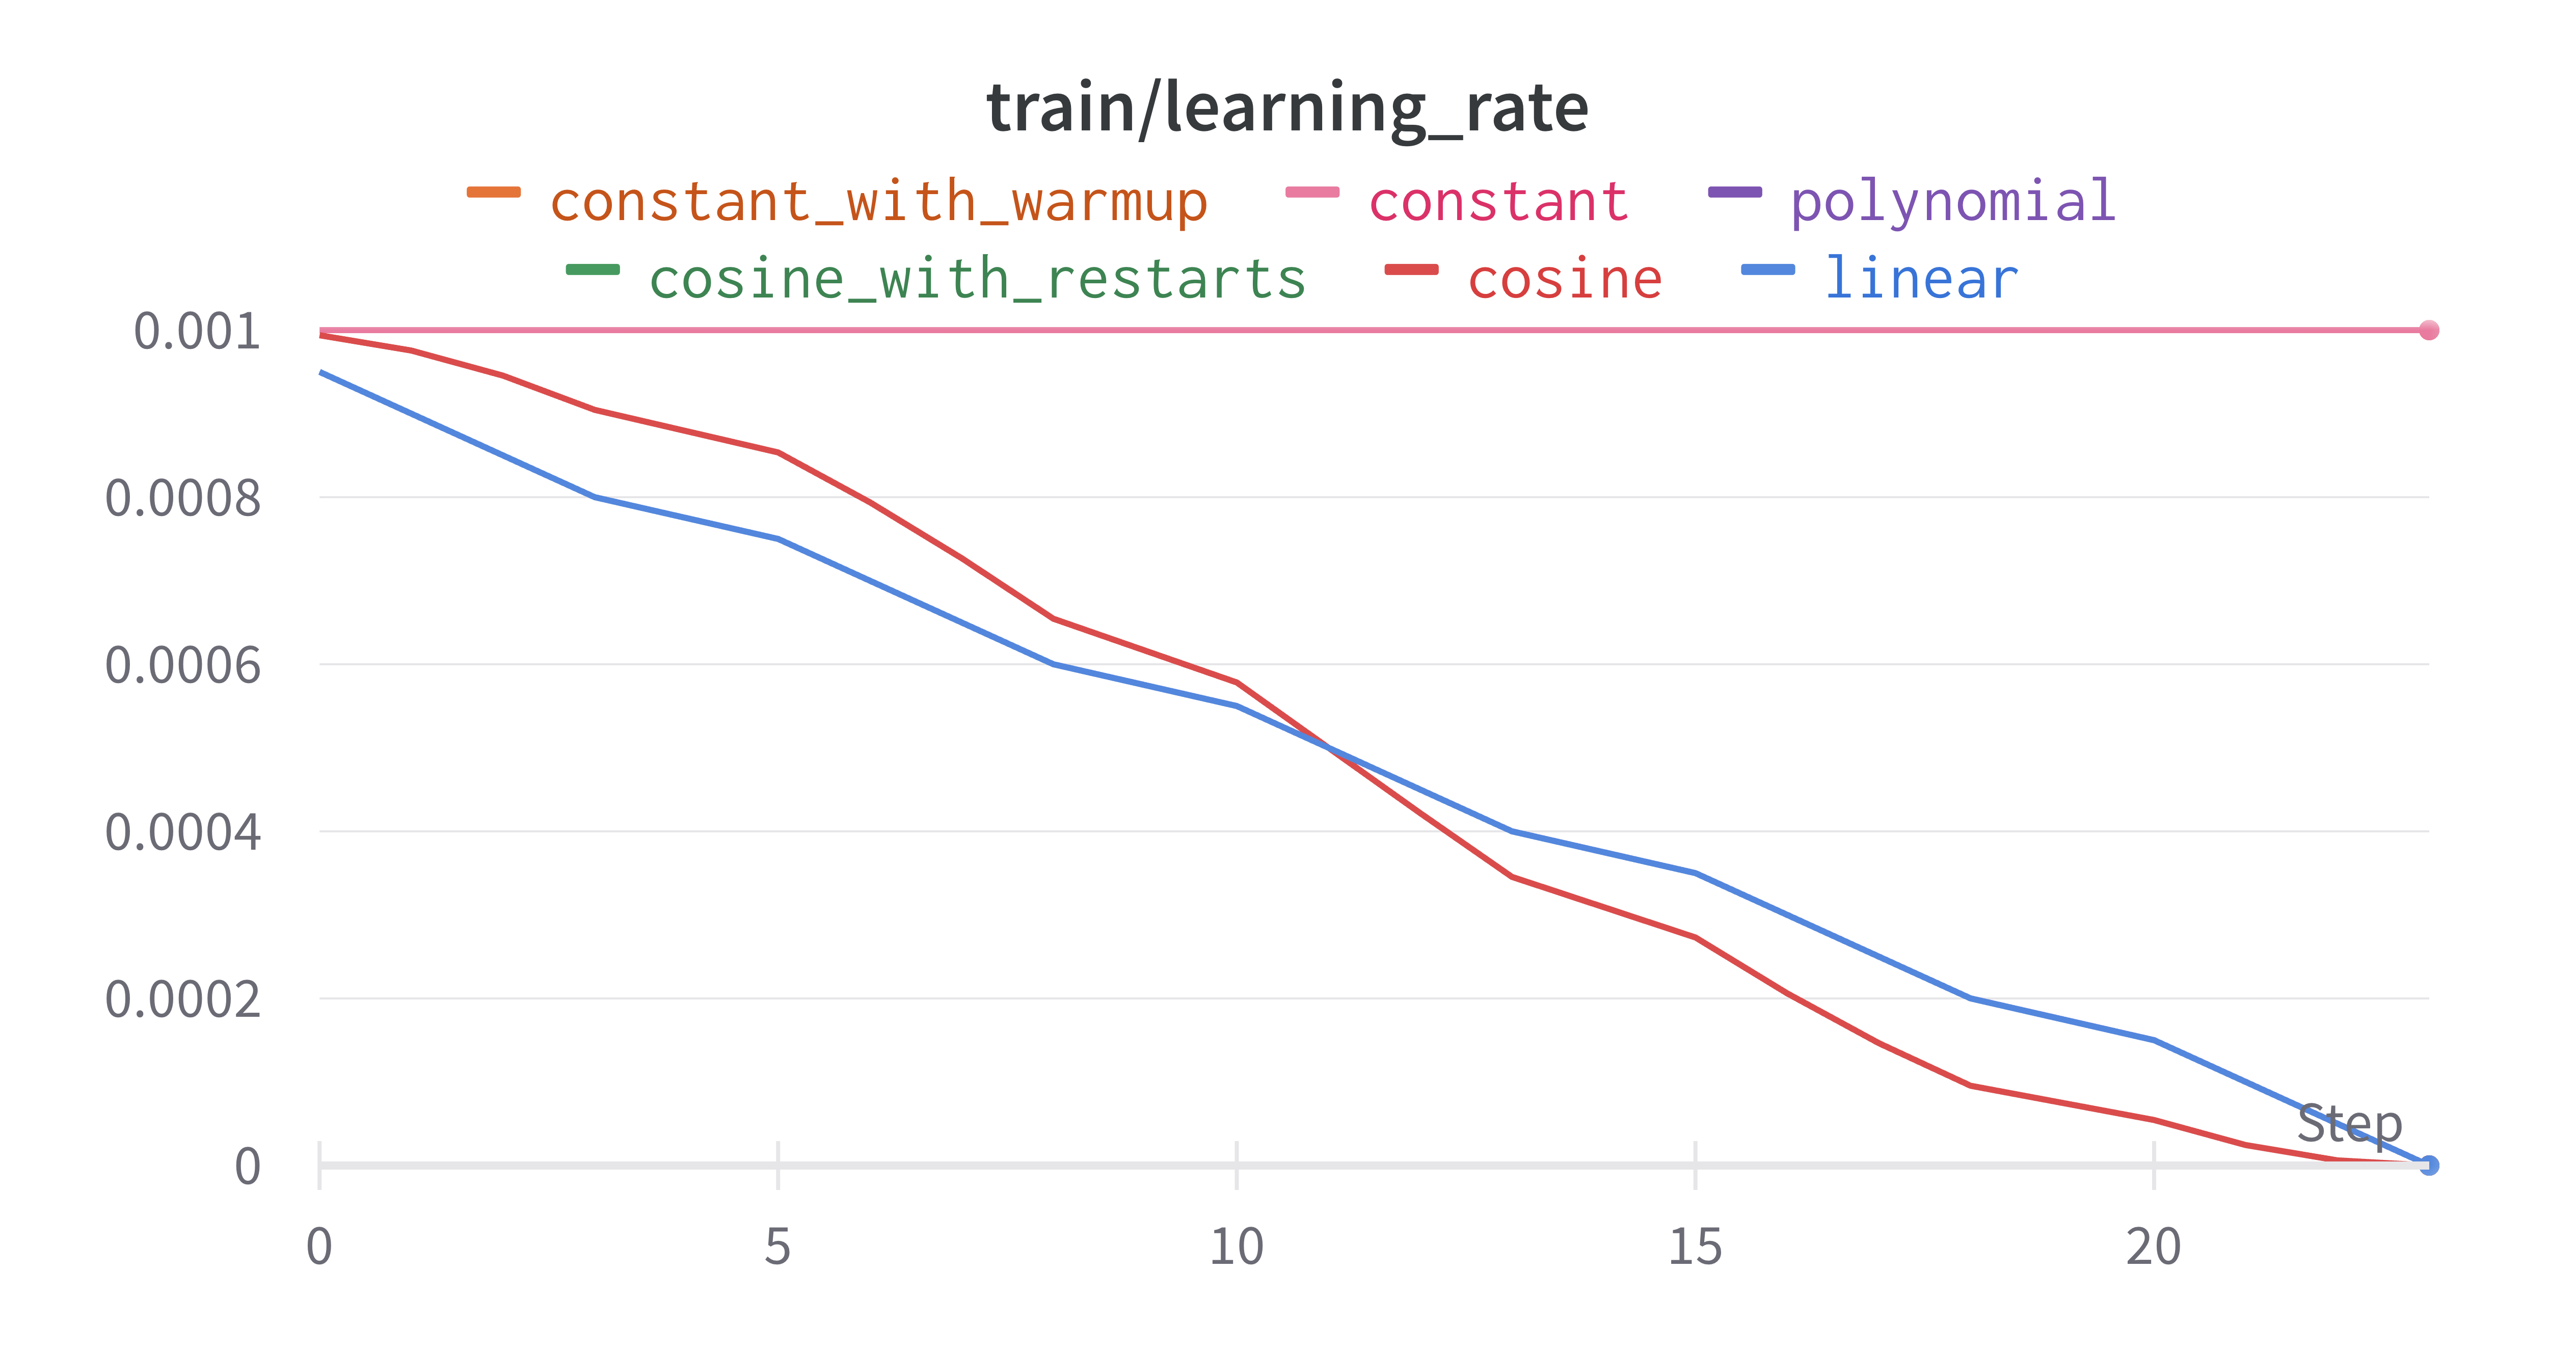
\includegraphics[width=.6\textwidth]{lr-s-lr}
  \caption{График изменения скорости обучения}
  \label{lr-s-lr}
\end{figure}

В следующих экспериментах при зафиксированном константном планировщике скорости обучения искалась наиболее эффективная скорость обучения. Стоит отметить, что при скорости обучения равной $1 \times 10^{-4}$ процесс обучения не завершился успешно. Из рисунков \ref{lr-train-loss}, \ref{lr-eval-loss}, \ref{lr-em}, \ref{lr-mauve} видно, что значения, близкие к $4 \times 10^{-4}$ и к $9 \times 10^{-4}$ показывают лучшие значения функций ошибок на всех выборках и лучшие значения метрик. Значение скорости обучения $9 \times 10^{-4}$ показывает результаты чуть лучше, чем $4 \times 10^{-4}$, быстрее достигая лучших значений. В целом, почти все значения скорости обучения показывают схожие результаты, но выбор оптимальных параметров для обучения на большей выборке может сказаться на качестве модели.

% LR
\begin{figure}[!ht]
  \centering
  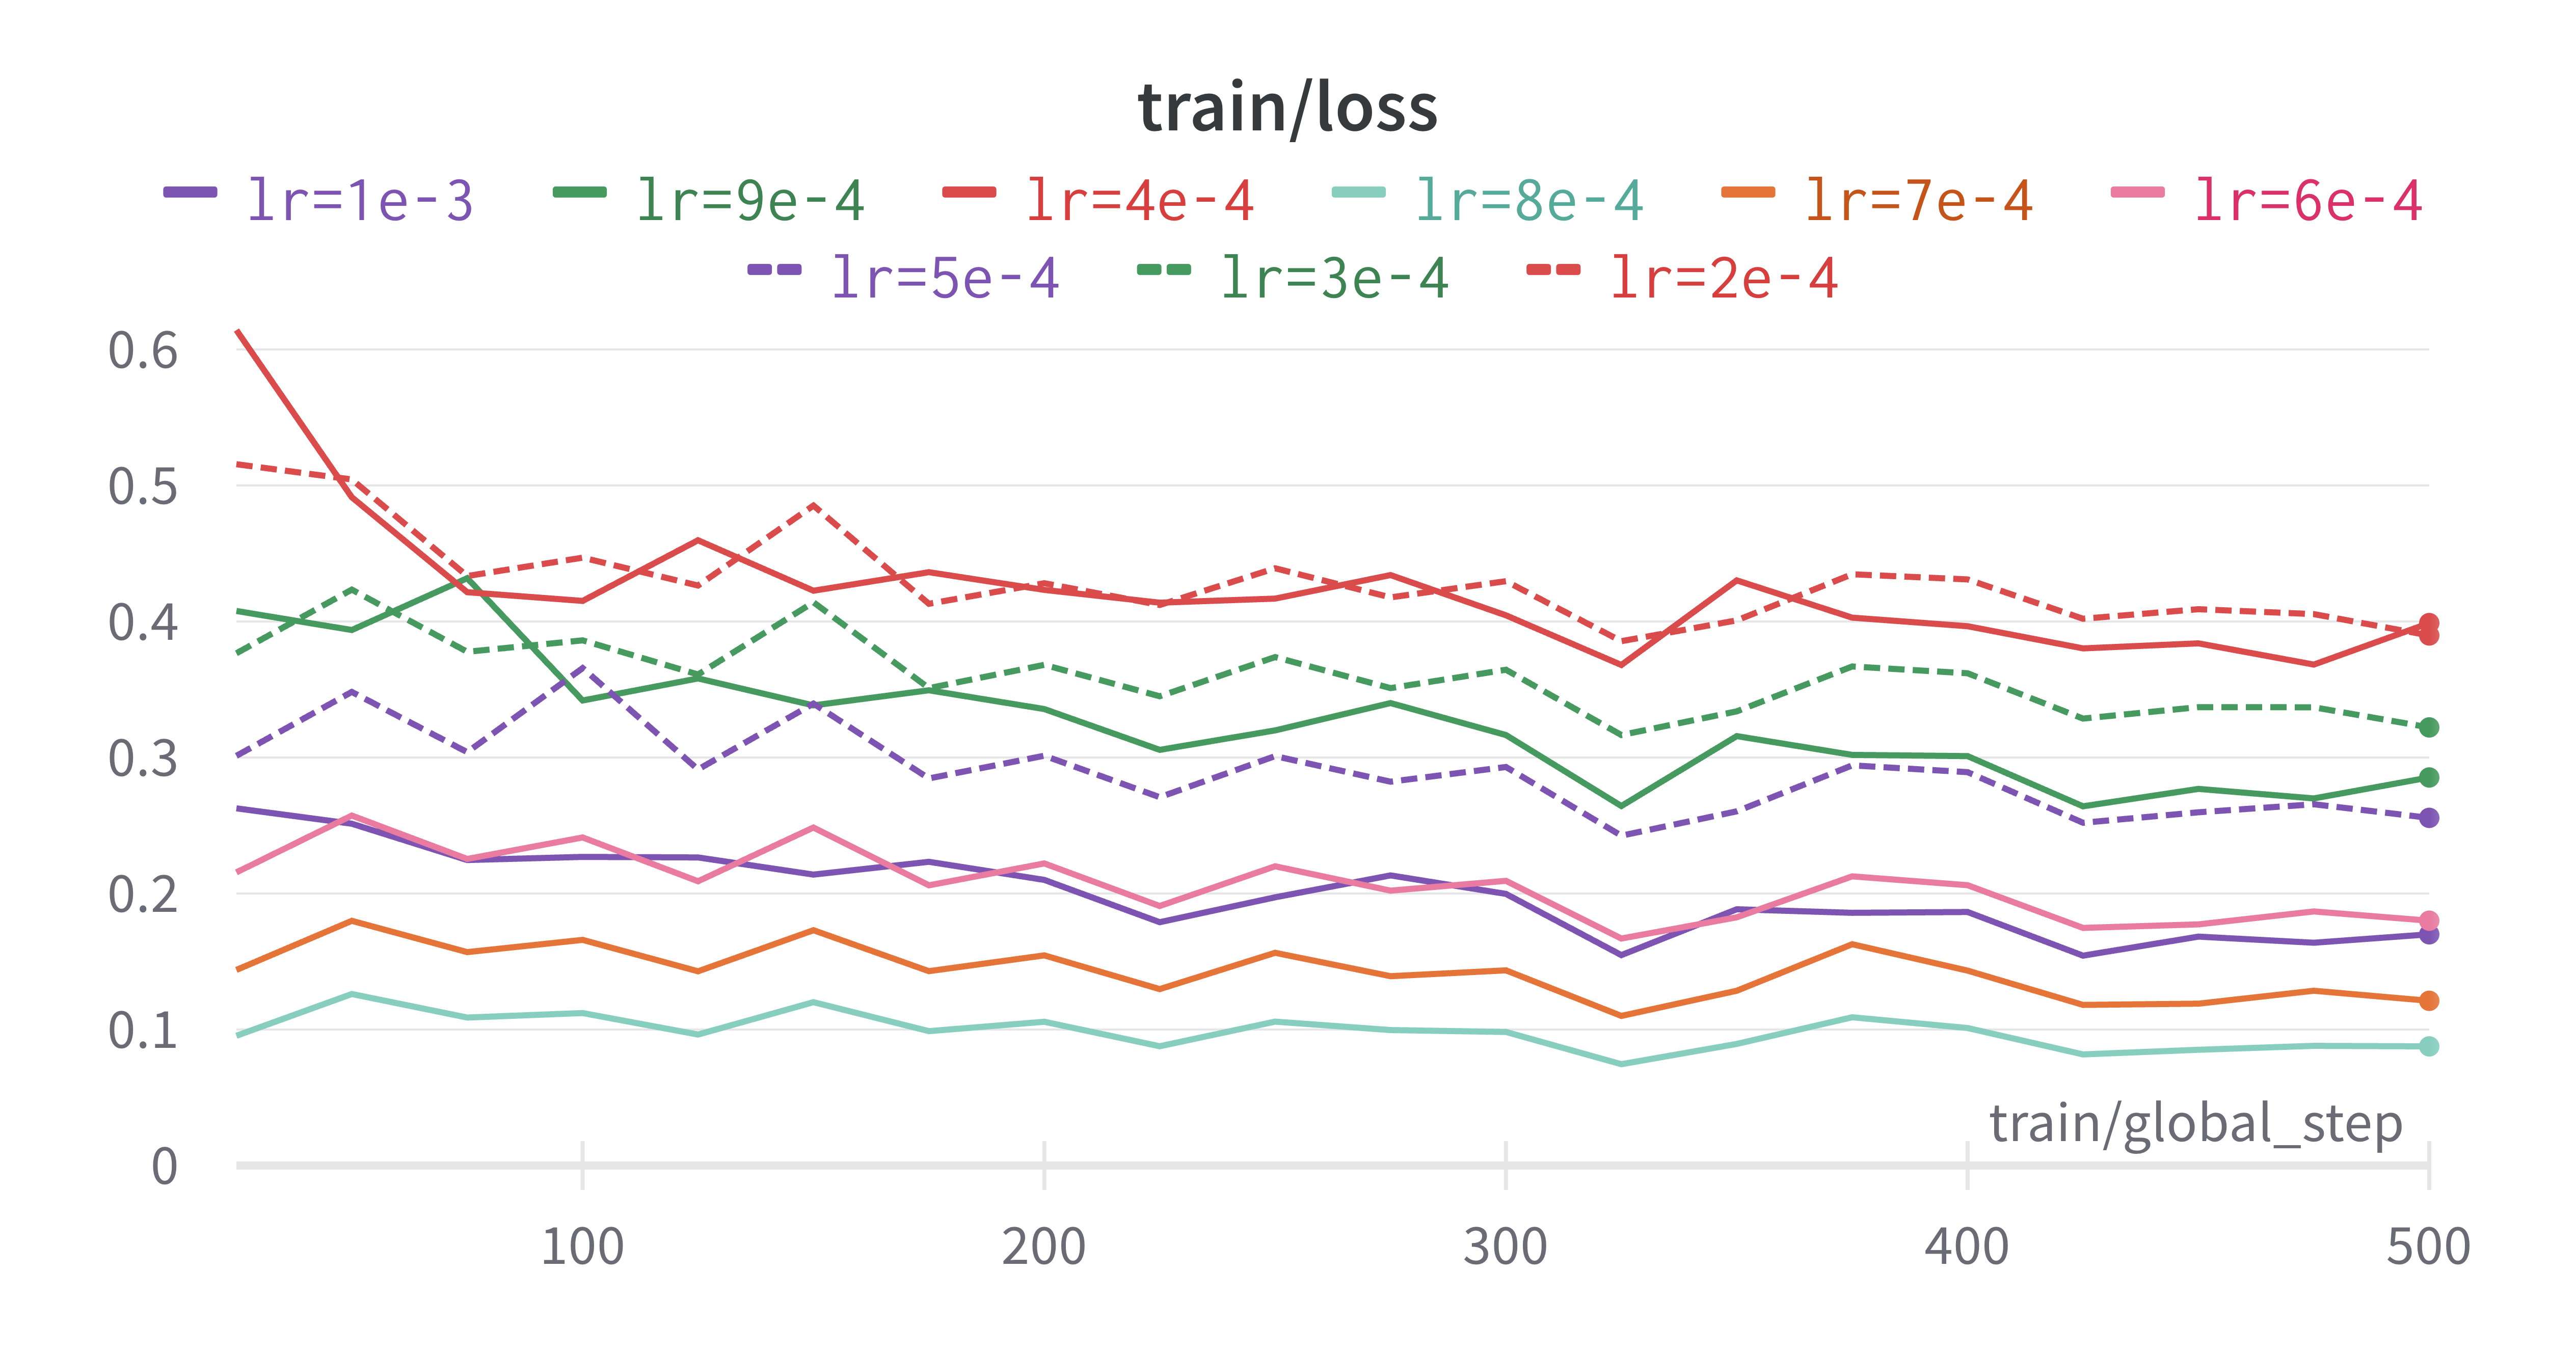
\includegraphics[width=.6\textwidth]{lr-train-loss}
  \caption{Значение функции ошибки на тренировочных данных}
  \label{lr-train-loss}
\end{figure}

\begin{figure}[!ht]
  \centering
  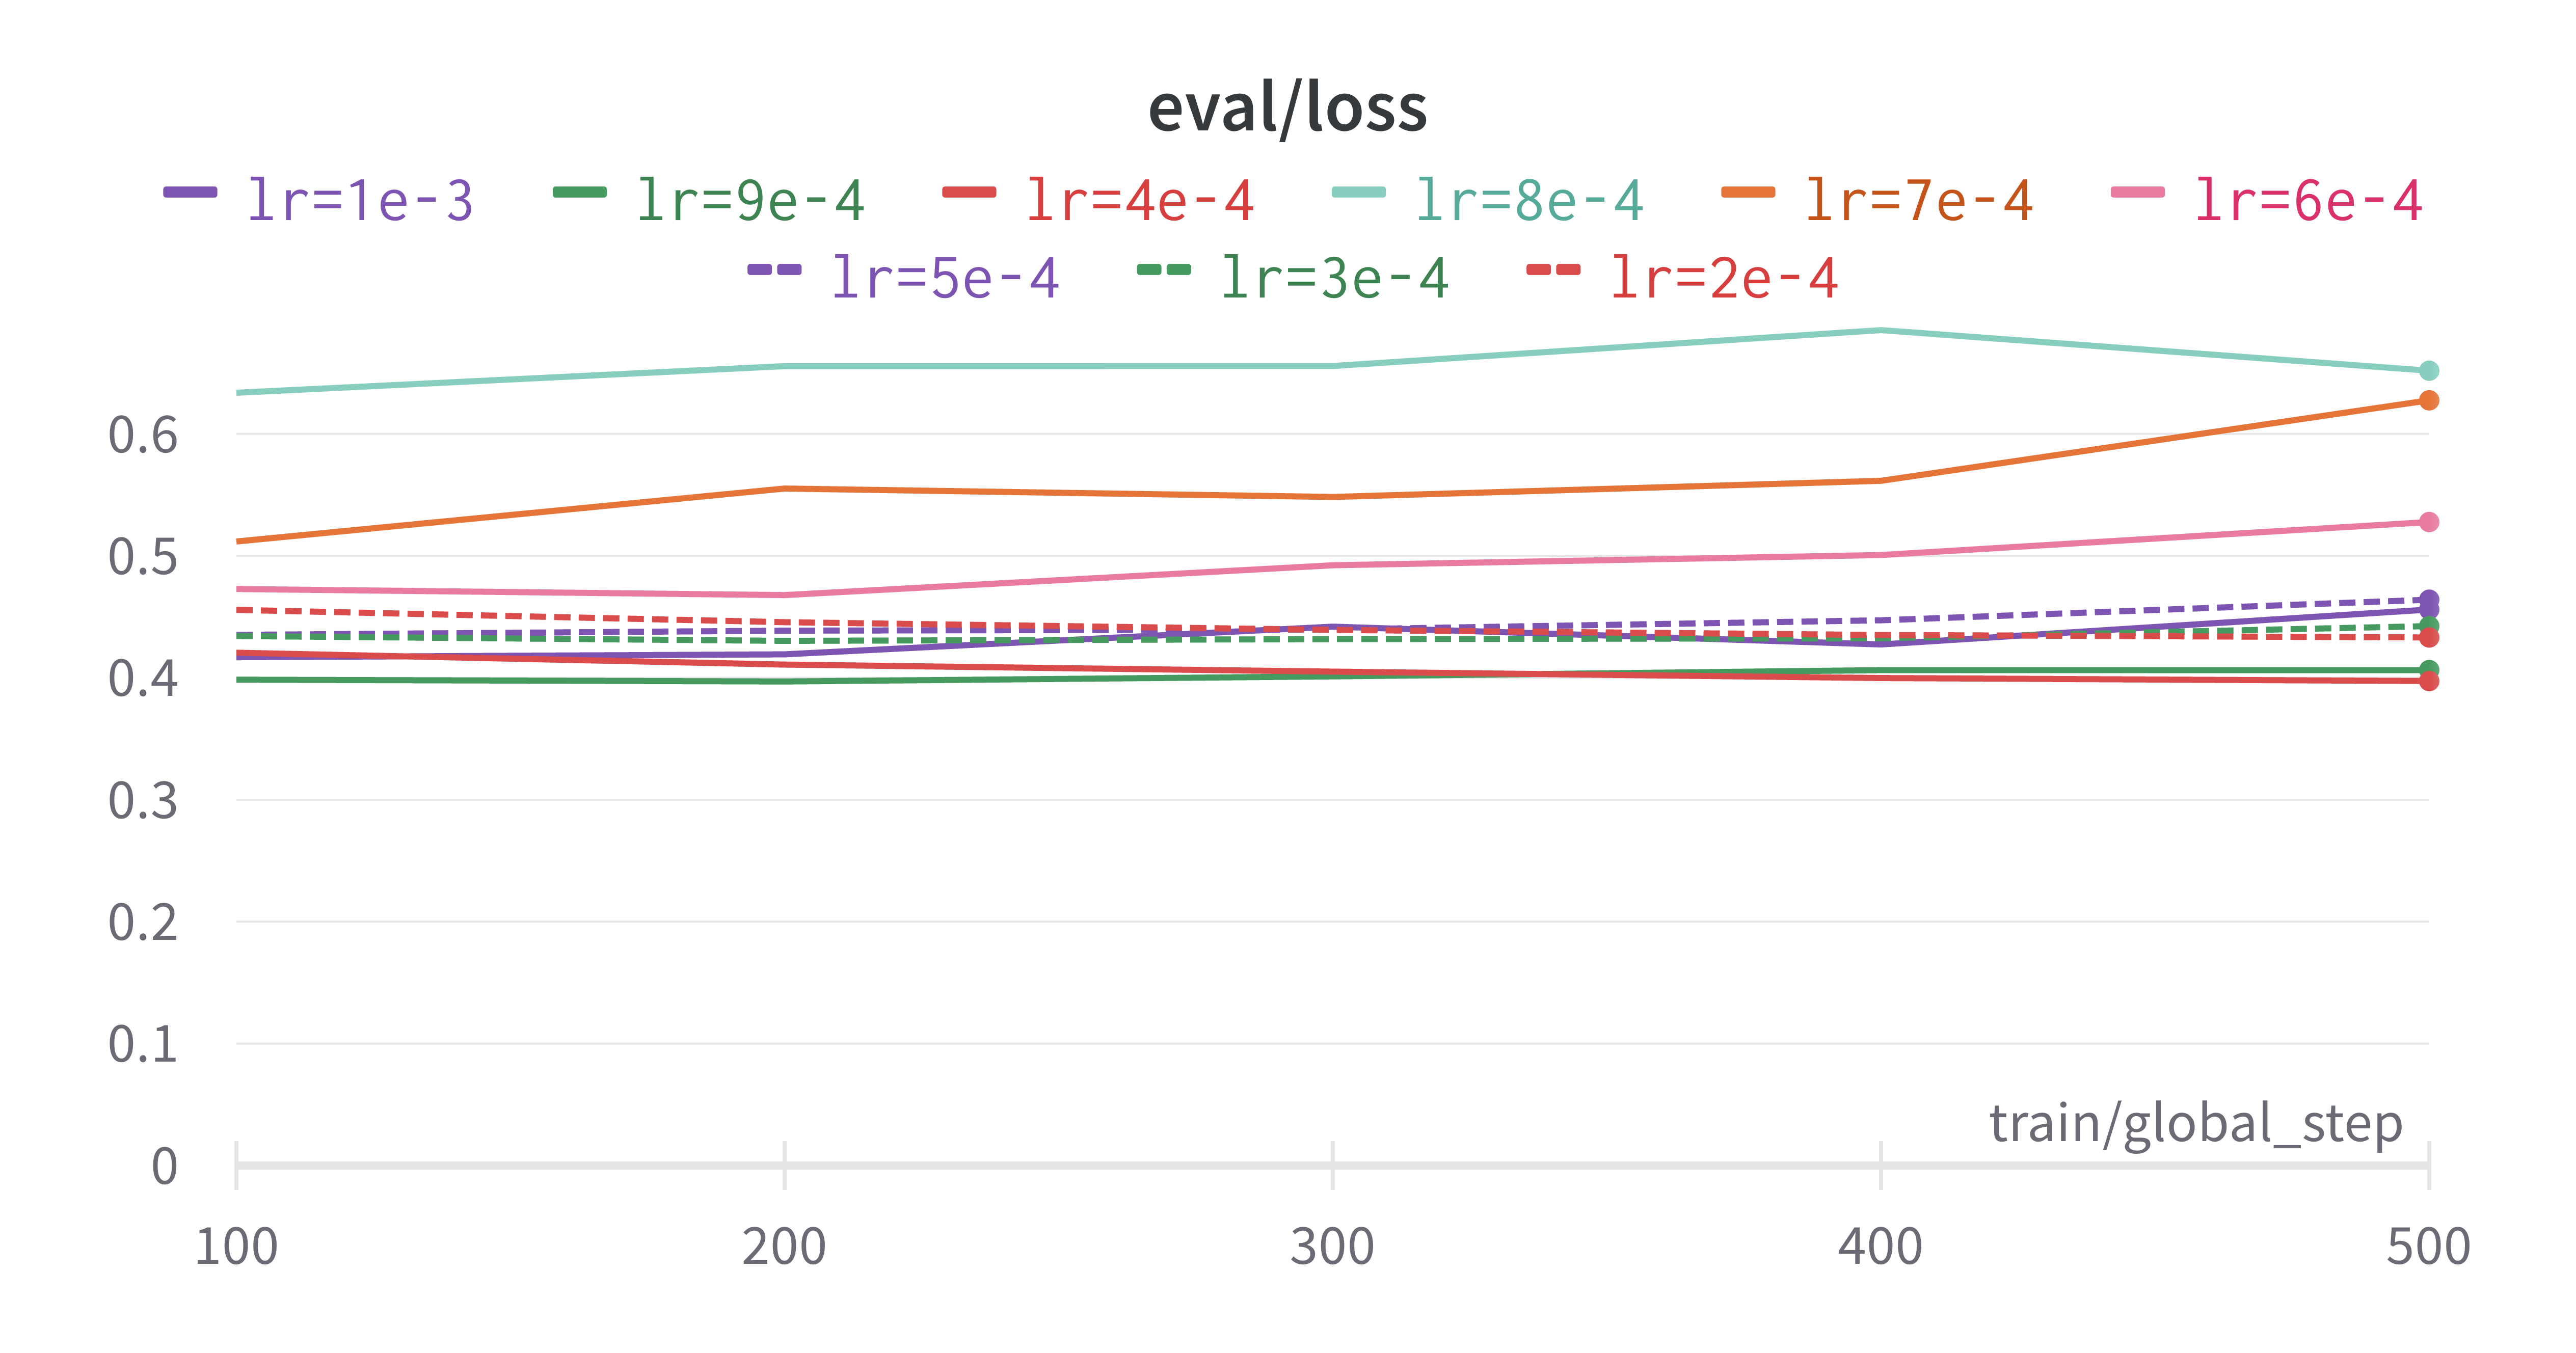
\includegraphics[width=.6\textwidth]{lr-eval-loss}
  \caption{Значение функции ошибки на валидационных данных}
  \label{lr-eval-loss}
\end{figure}

\begin{figure}[!ht]
  \centering
  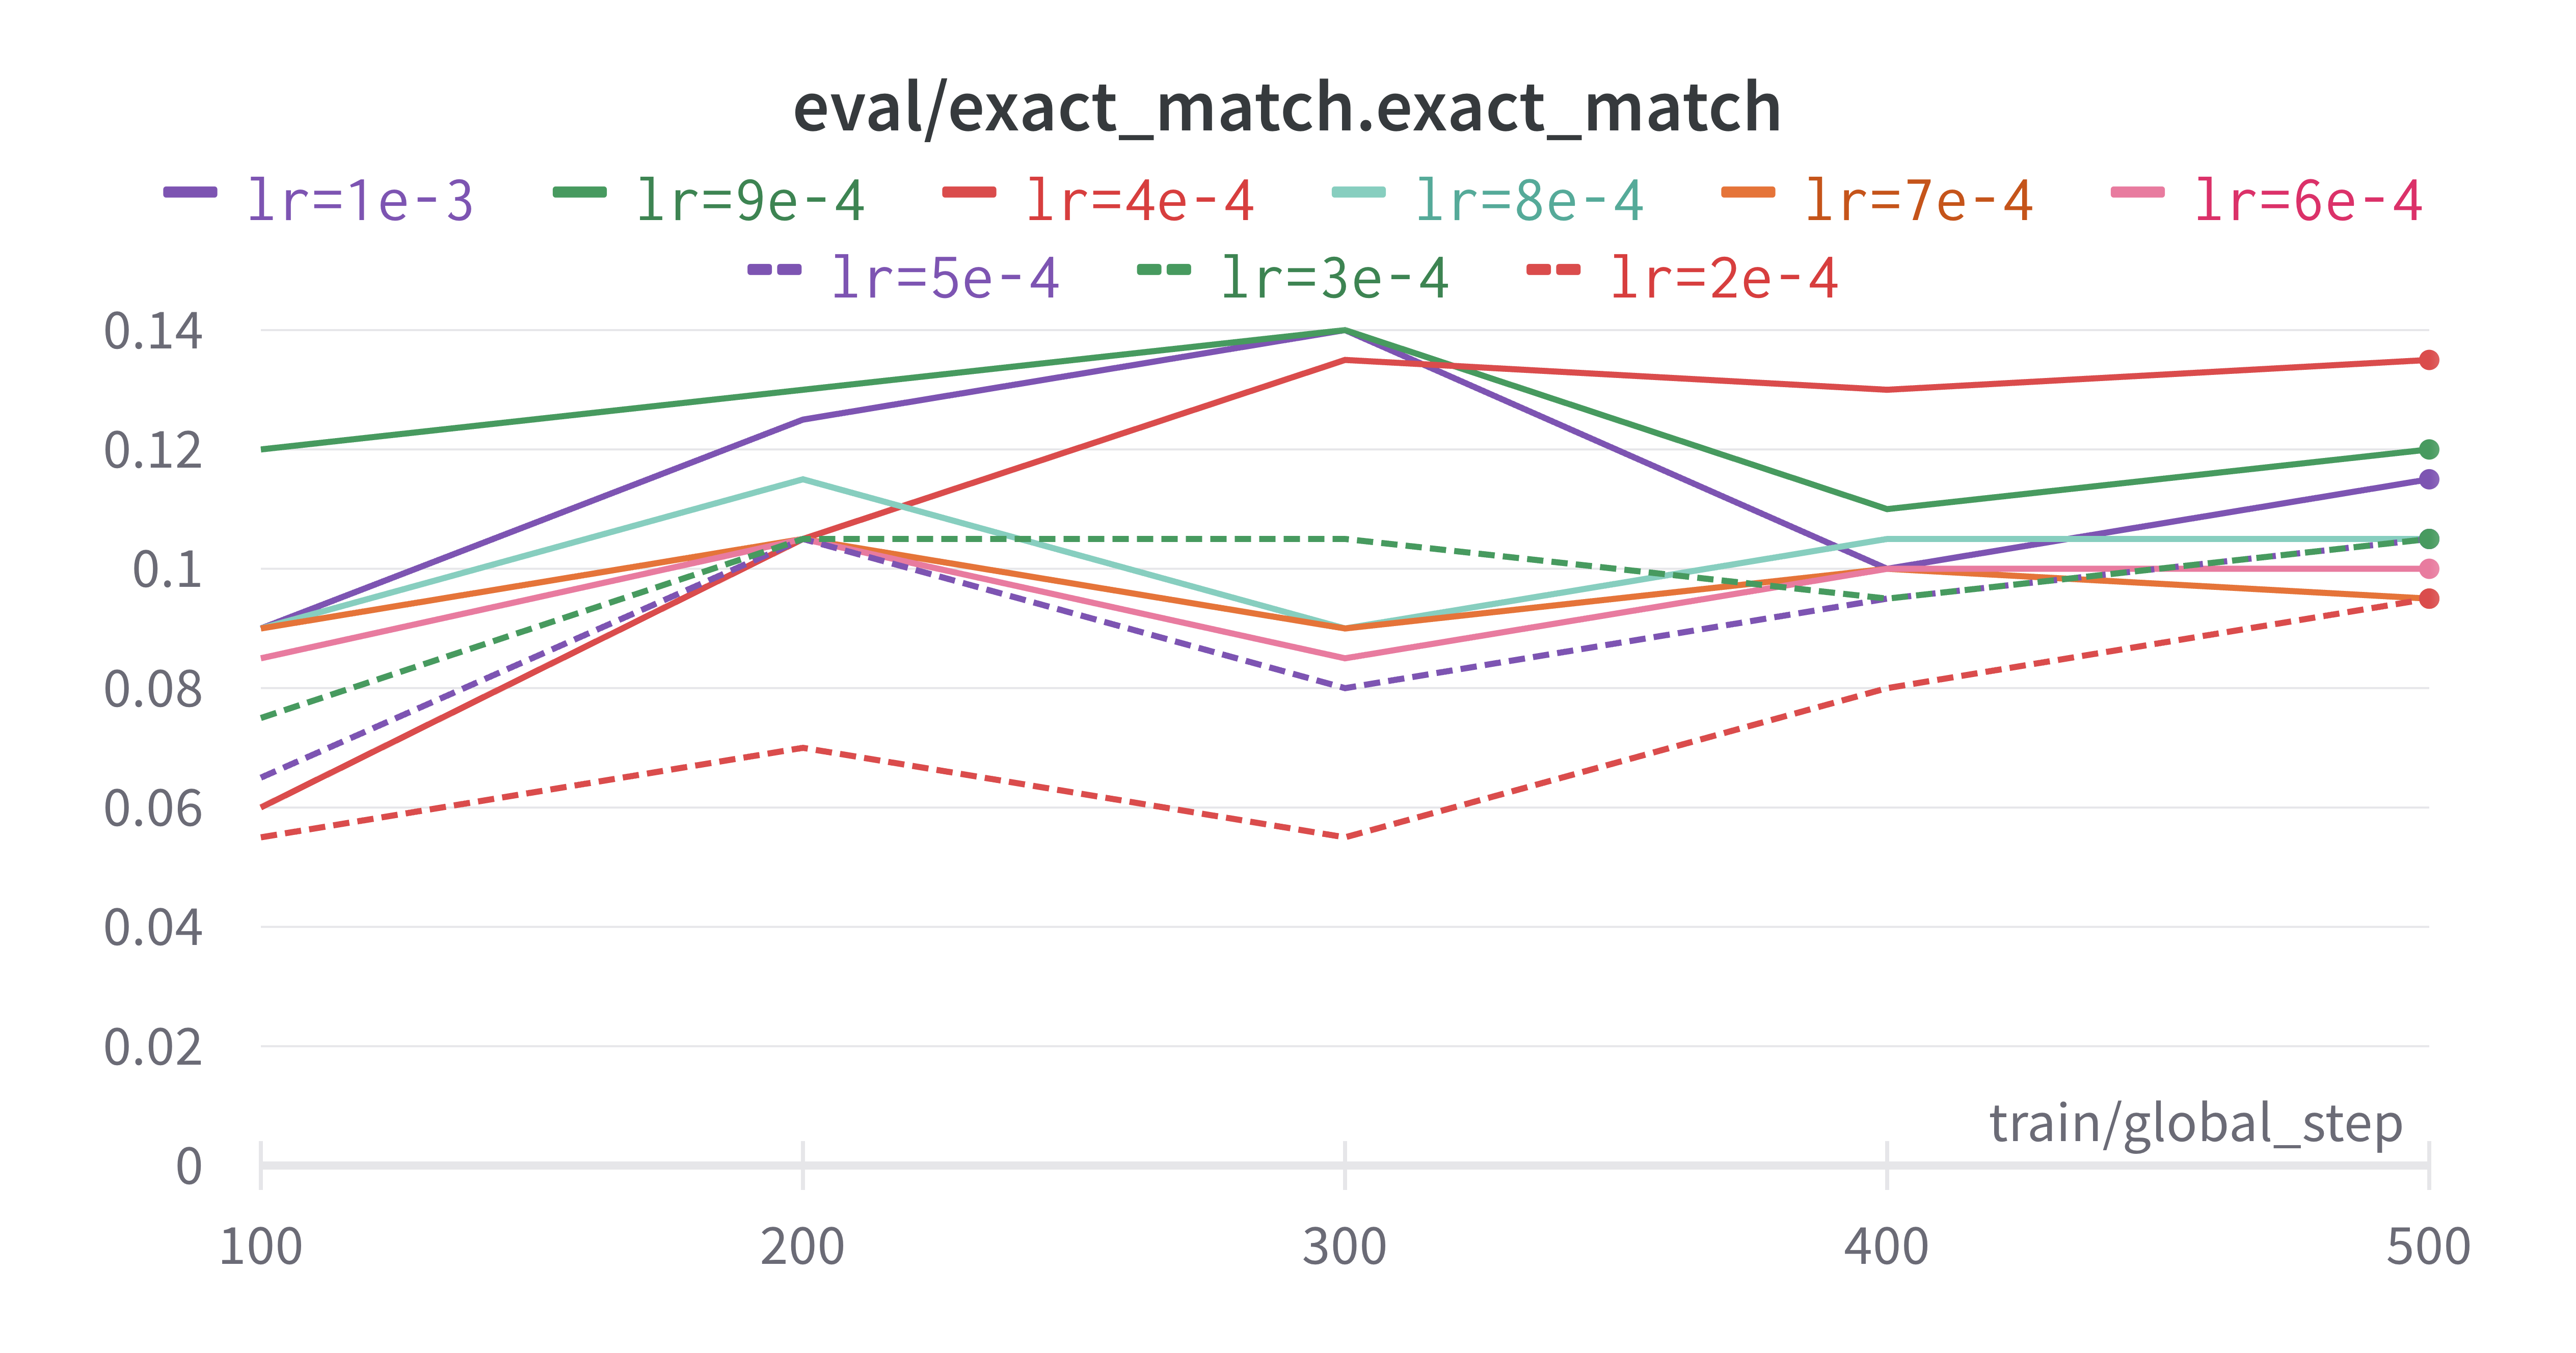
\includegraphics[width=.6\textwidth]{lr-em}
  \caption{Значение метрики Exact Match на валидационных данных}
  \label{lr-em}
\end{figure}

\begin{figure}[!ht]
  \centering
  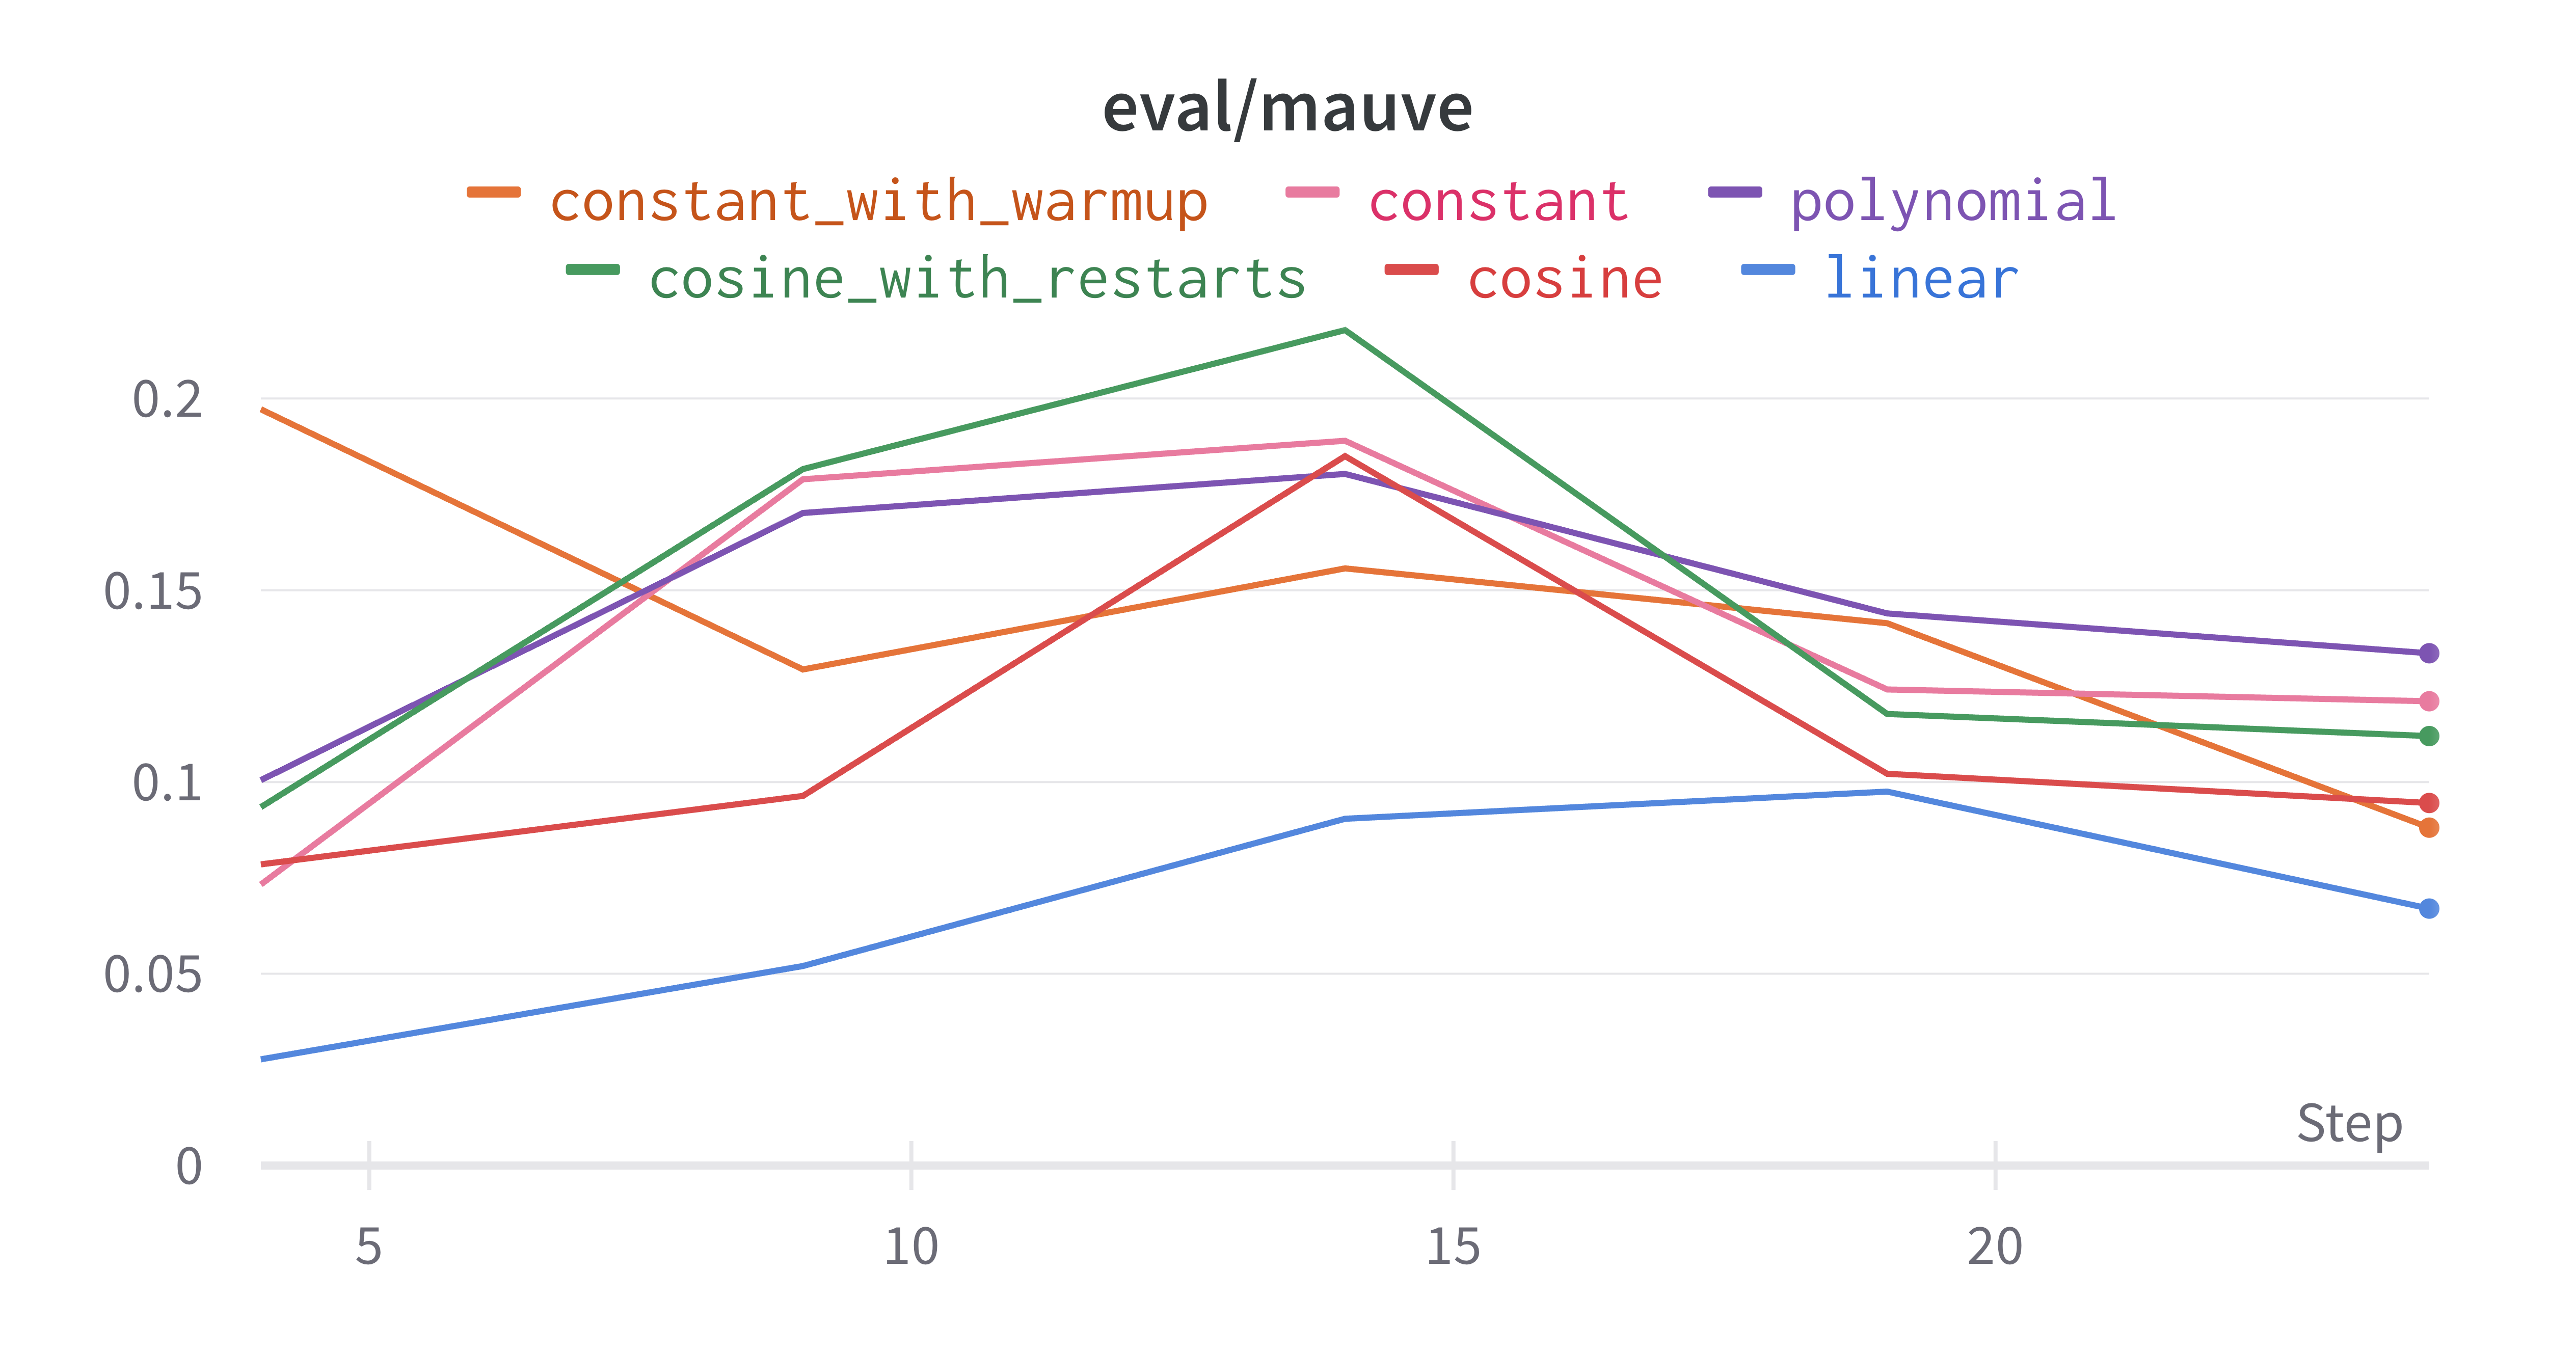
\includegraphics[width=.6\textwidth]{lr-s-mauve}
  \caption{Значение метрики MAUVE на валидационных данных}
  \label{lr-mauve}
\end{figure}

Исходя из всех экспериментов можно сделать вывод, что оптимальные параметры для обучения будут константный планировщик скорости обучения и скорость обучения со значением $9 \times 10{-4}$

\section{ОБУЧЕНИЕ ИТОГОВОЙ МОДЕЛИ}

С подобранными ранее параметрами на была обучена итоговая модель. Общее количество операций, произведенных во время обучения, составило $2 \times 10^{18}$. Количество токенов, которые фигурировали в процессе обучения -- $25 \times 10^{6}$. Процесс обучения виден на рисунках \ref{total-train-loss}, \ref{total-eval-loss}, \ref{total-em}, \ref{total-mauve}. Низкие значения метрик Exact Match и MAUVE можно объяснить сложностью поставленной модели задачи: в диалогах часто ответы формируются исходя из внешних условий, в которых происходился диалог с неигровым персонажем, которые сложно получить из данных игры в формате естественного языка. Метрика Exact Match довольно грубо оценивает результат генерации -- переформулированная фраза в такой оценке даст значение 0. Тем не менее, такую систему получилось обучить на потребительском оборудовании на неплохие результаты. Далее идет пример диалога, который был произведен с моделью.

\texttt{\\Below is the definition of in-game NPC.\\
  The Mad Lord\\
  Alignment: Chaotic Neutral\\
  Description: A mysterious figure who resides in a castle called Caste Maluradek in the middle of a forest. He is a powerful wizard who has the ability to manipulate the elements and create illusions.\\
  Personality traits: He is obsessed with power and will stop at nothing to achieve his goals.\\
  Flaws: He wants to prove that he is the most powerful wizard in the world.
  Motivation: The Mad Lord is a mysterious figure who is driven by his desire for power. He is a master manipulator and will use any means necessary to achieve his goals. He is a powerful wizard who is not afraid to use his magic to get what he wants. He is also a bit of a showman, as he enjoys creating elaborate illusions to impress his guests.\\
  Dialogue history:\\
  Player: START DIALOGUE\\
  NPC: Salutations to the travelers. Welcome to Castle Maluradek. I am your adversary.\\
  Player query: Does the adversary have a name?\\
  Respond to player's query based on defined NPC:\\
  ANSWER: I do not have a name. I am a practitioner of magic. I work in the fields of the great forest.}

Больше примеров можно увидеть в приложении \ref{app:diagogue}.

\begin{figure}[!ht]
  \centering
  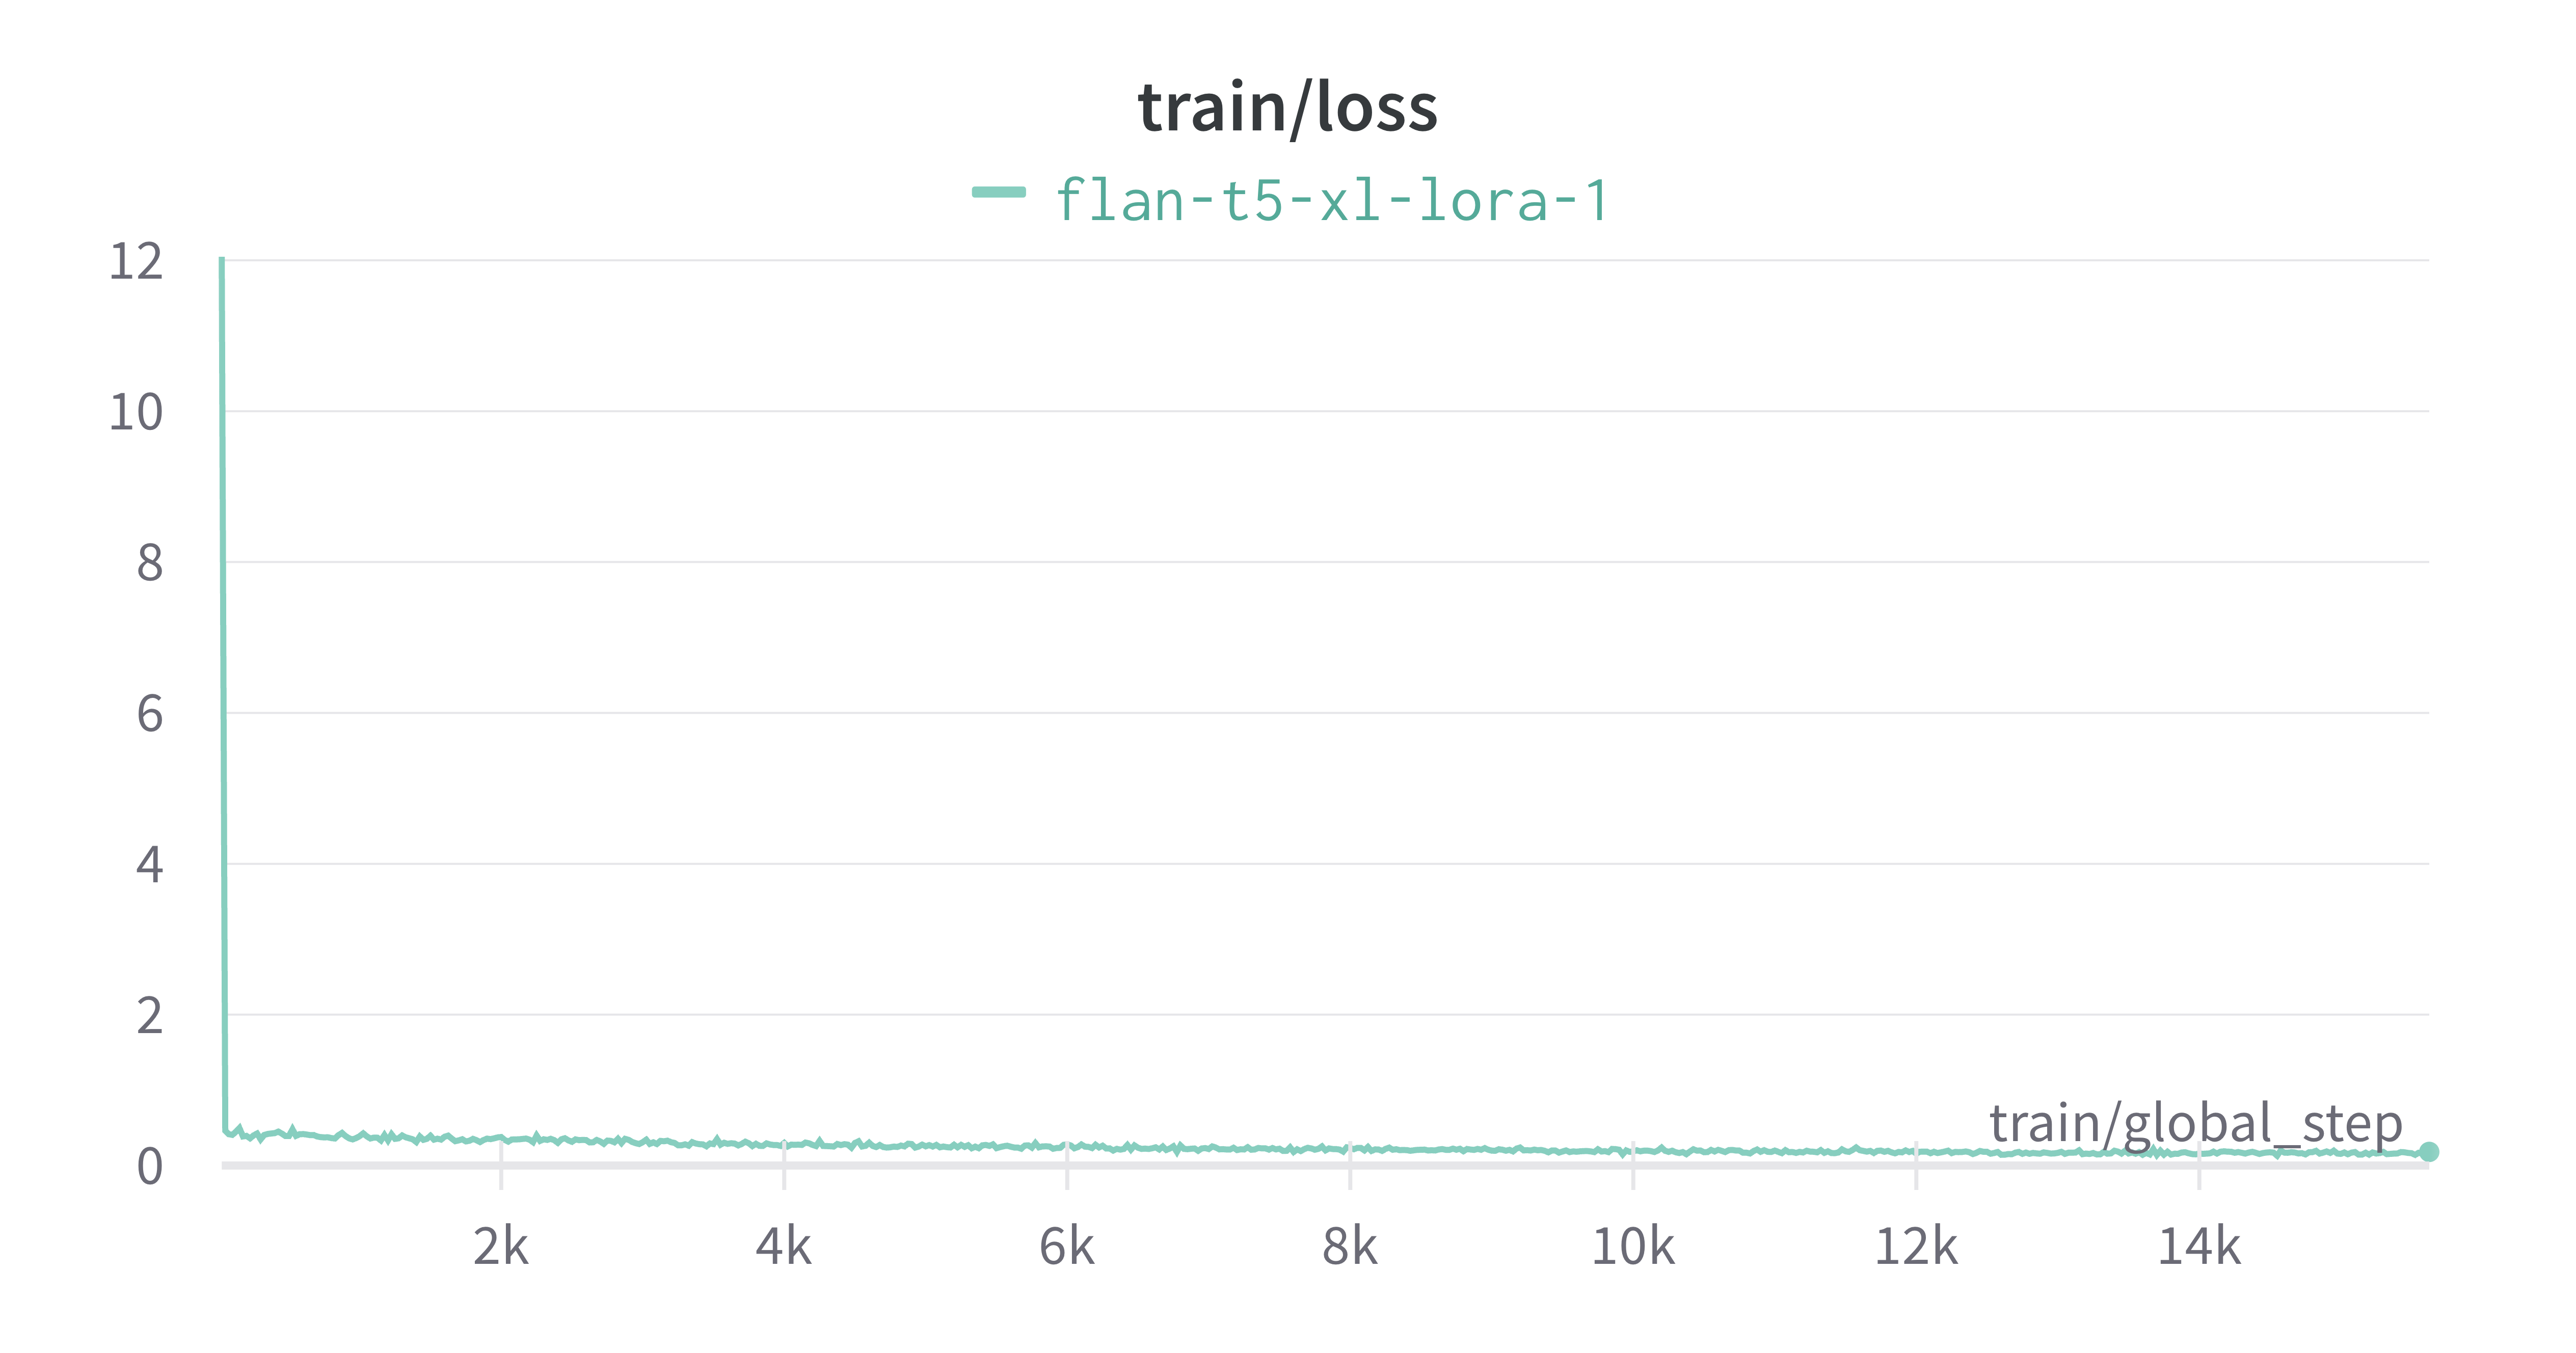
\includegraphics[width=.6\textwidth]{total-train-loss}
  \caption{Значение функции ошибки на тренировочных данных}
  \label{total-train-loss}
\end{figure}

\begin{figure}[!ht]
  \centering
  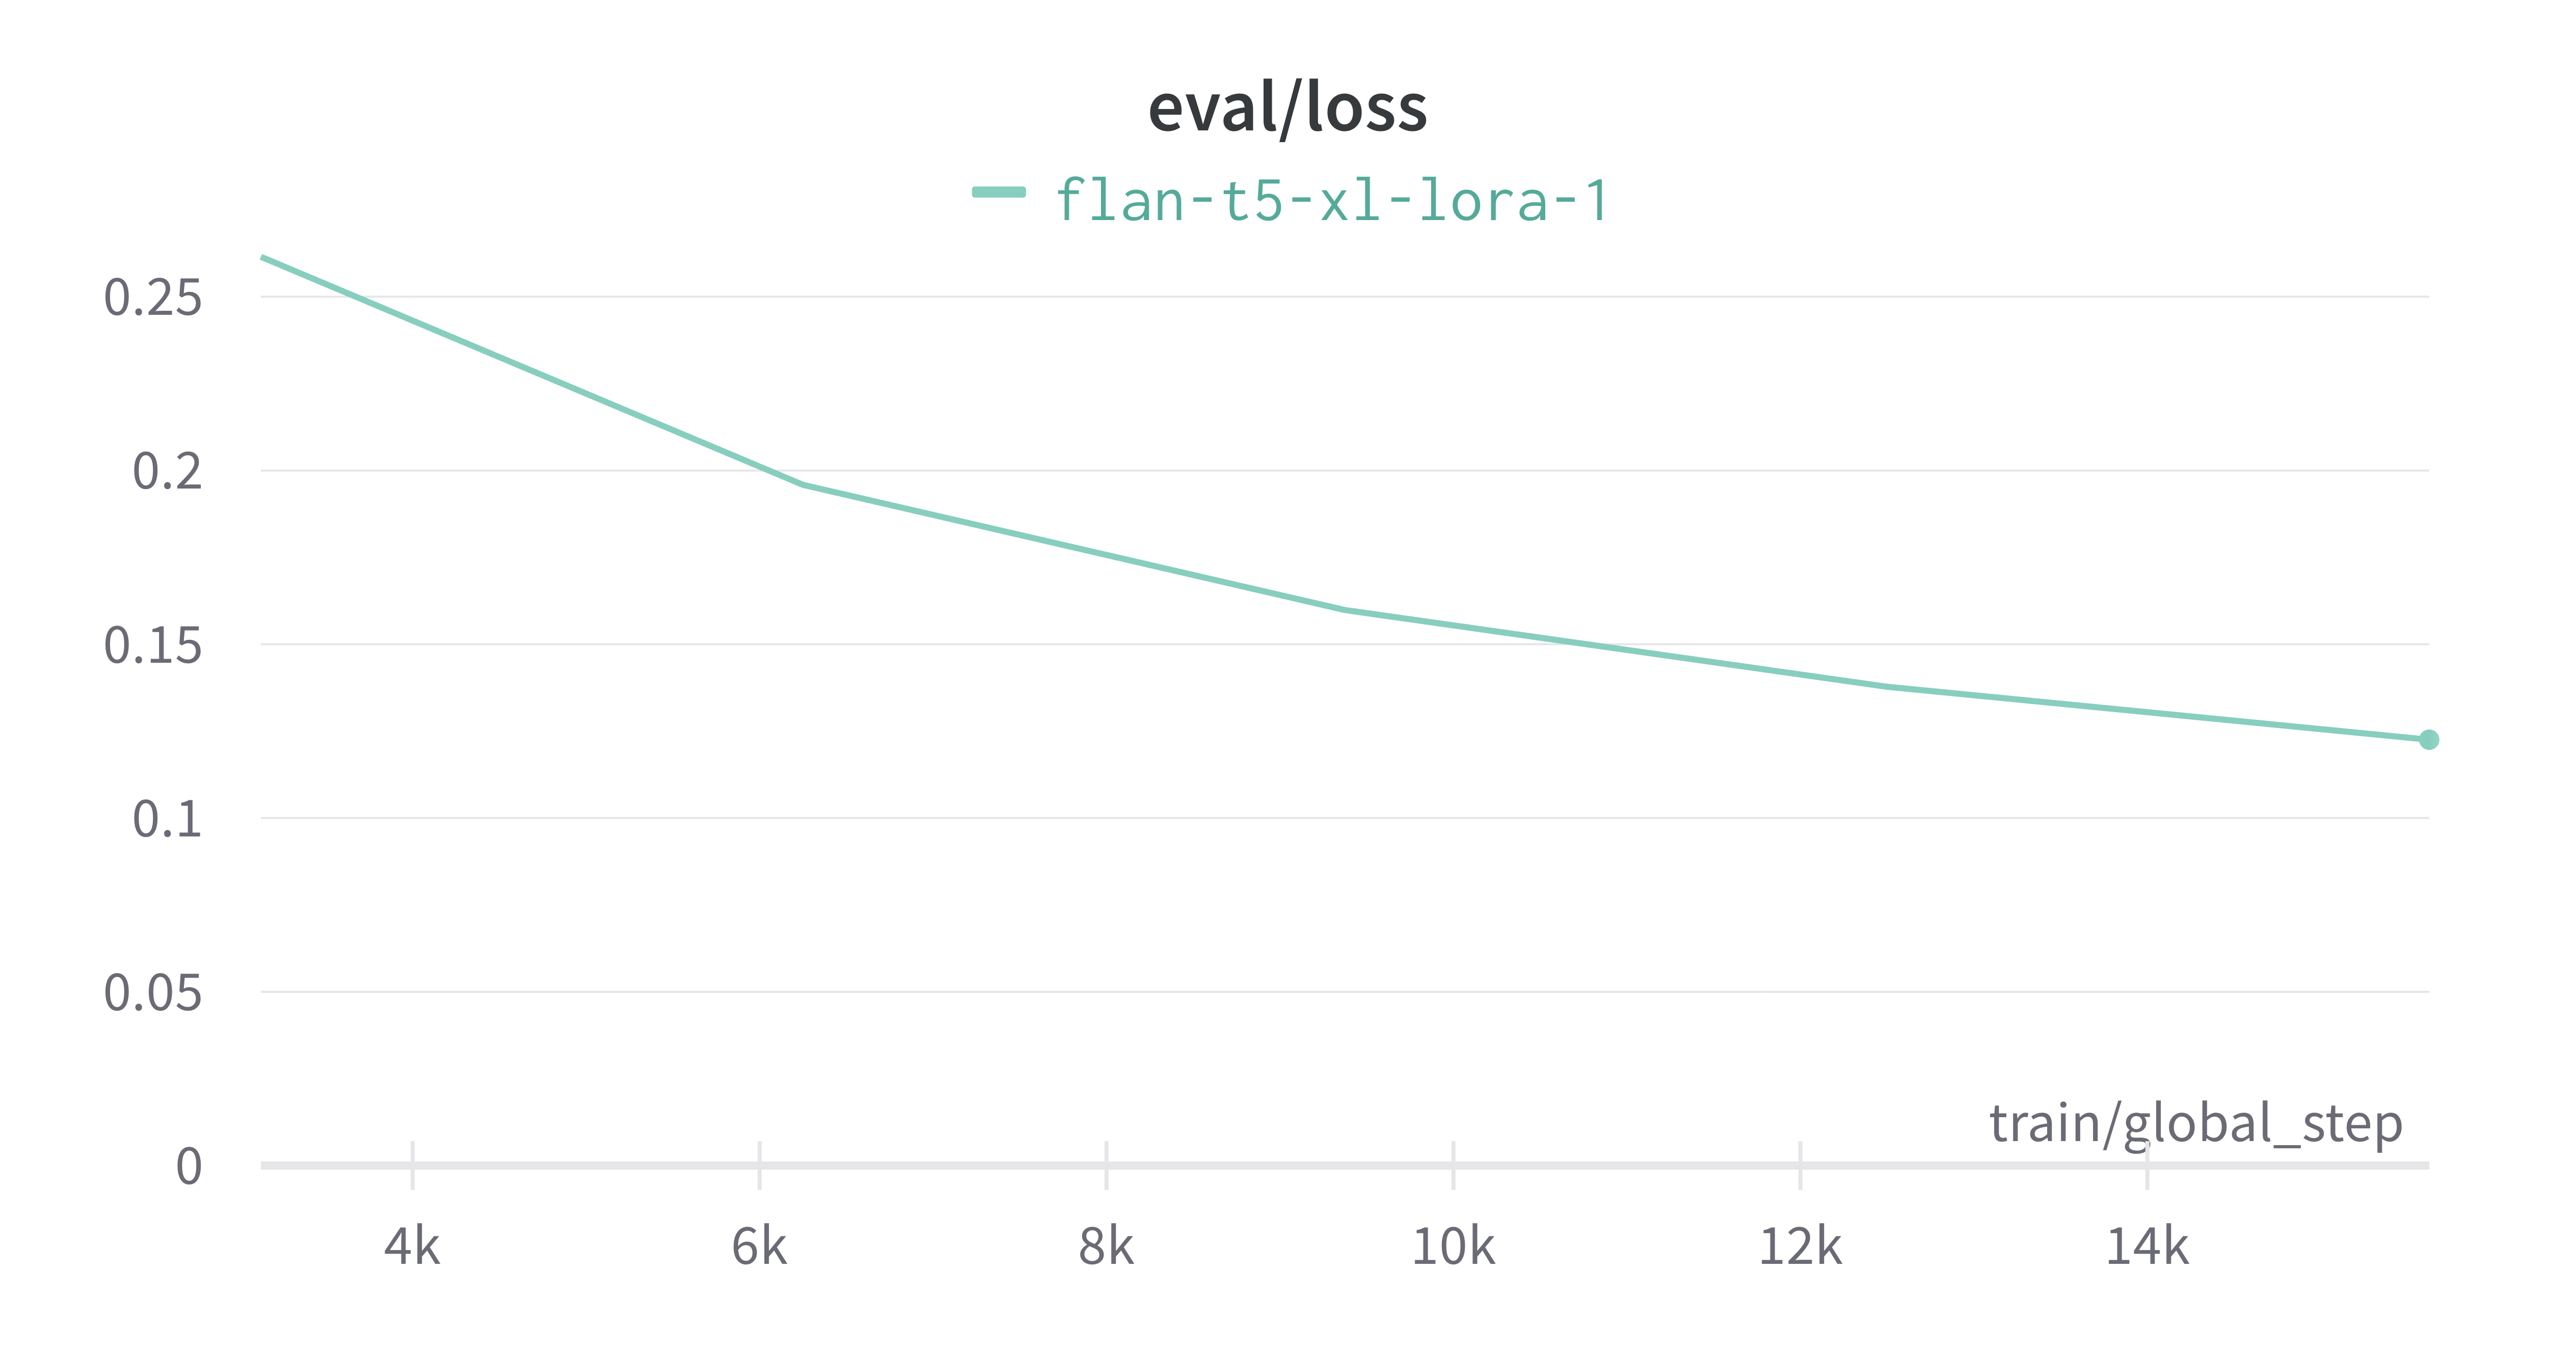
\includegraphics[width=.6\textwidth]{total-eval-loss}
  \caption{Значение функции ошибки на валидационных данных}
  \label{total-eval-loss}
\end{figure}

\begin{figure}[!ht]
  \centering
  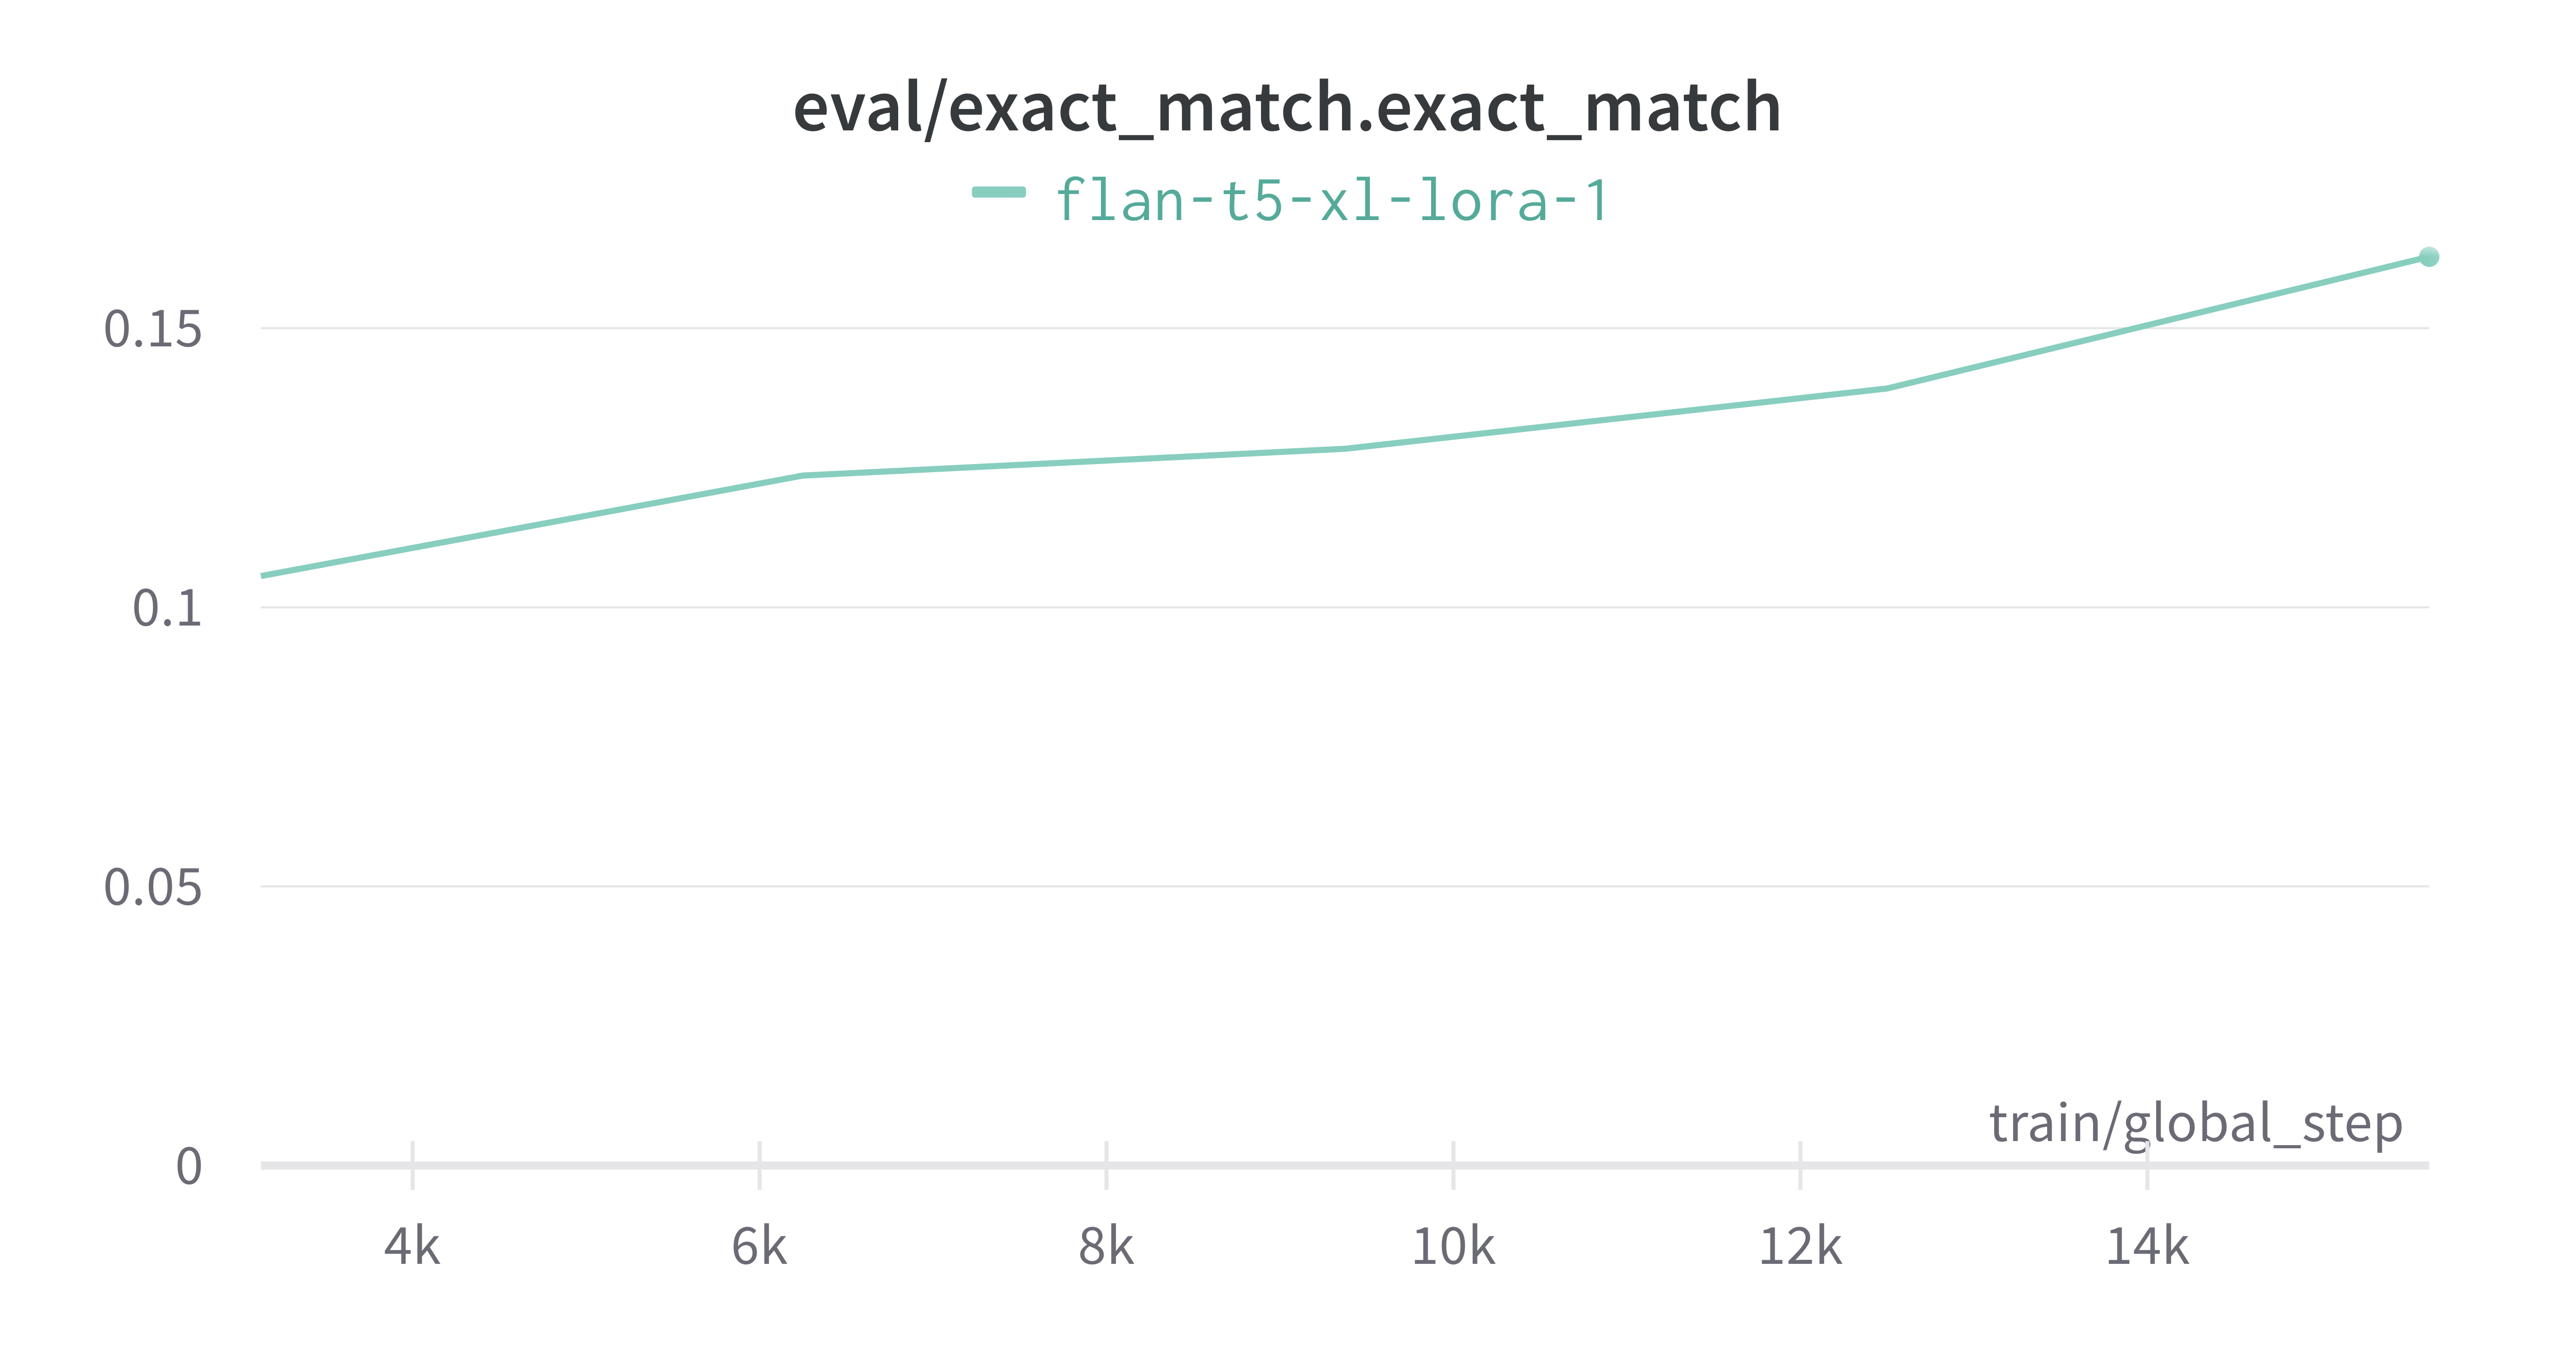
\includegraphics[width=.6\textwidth]{total-em}
  \caption{Значение метрики Exact Match на валидационных данных}
  \label{total-em}
\end{figure}

\begin{figure}[!ht]
  \centering
  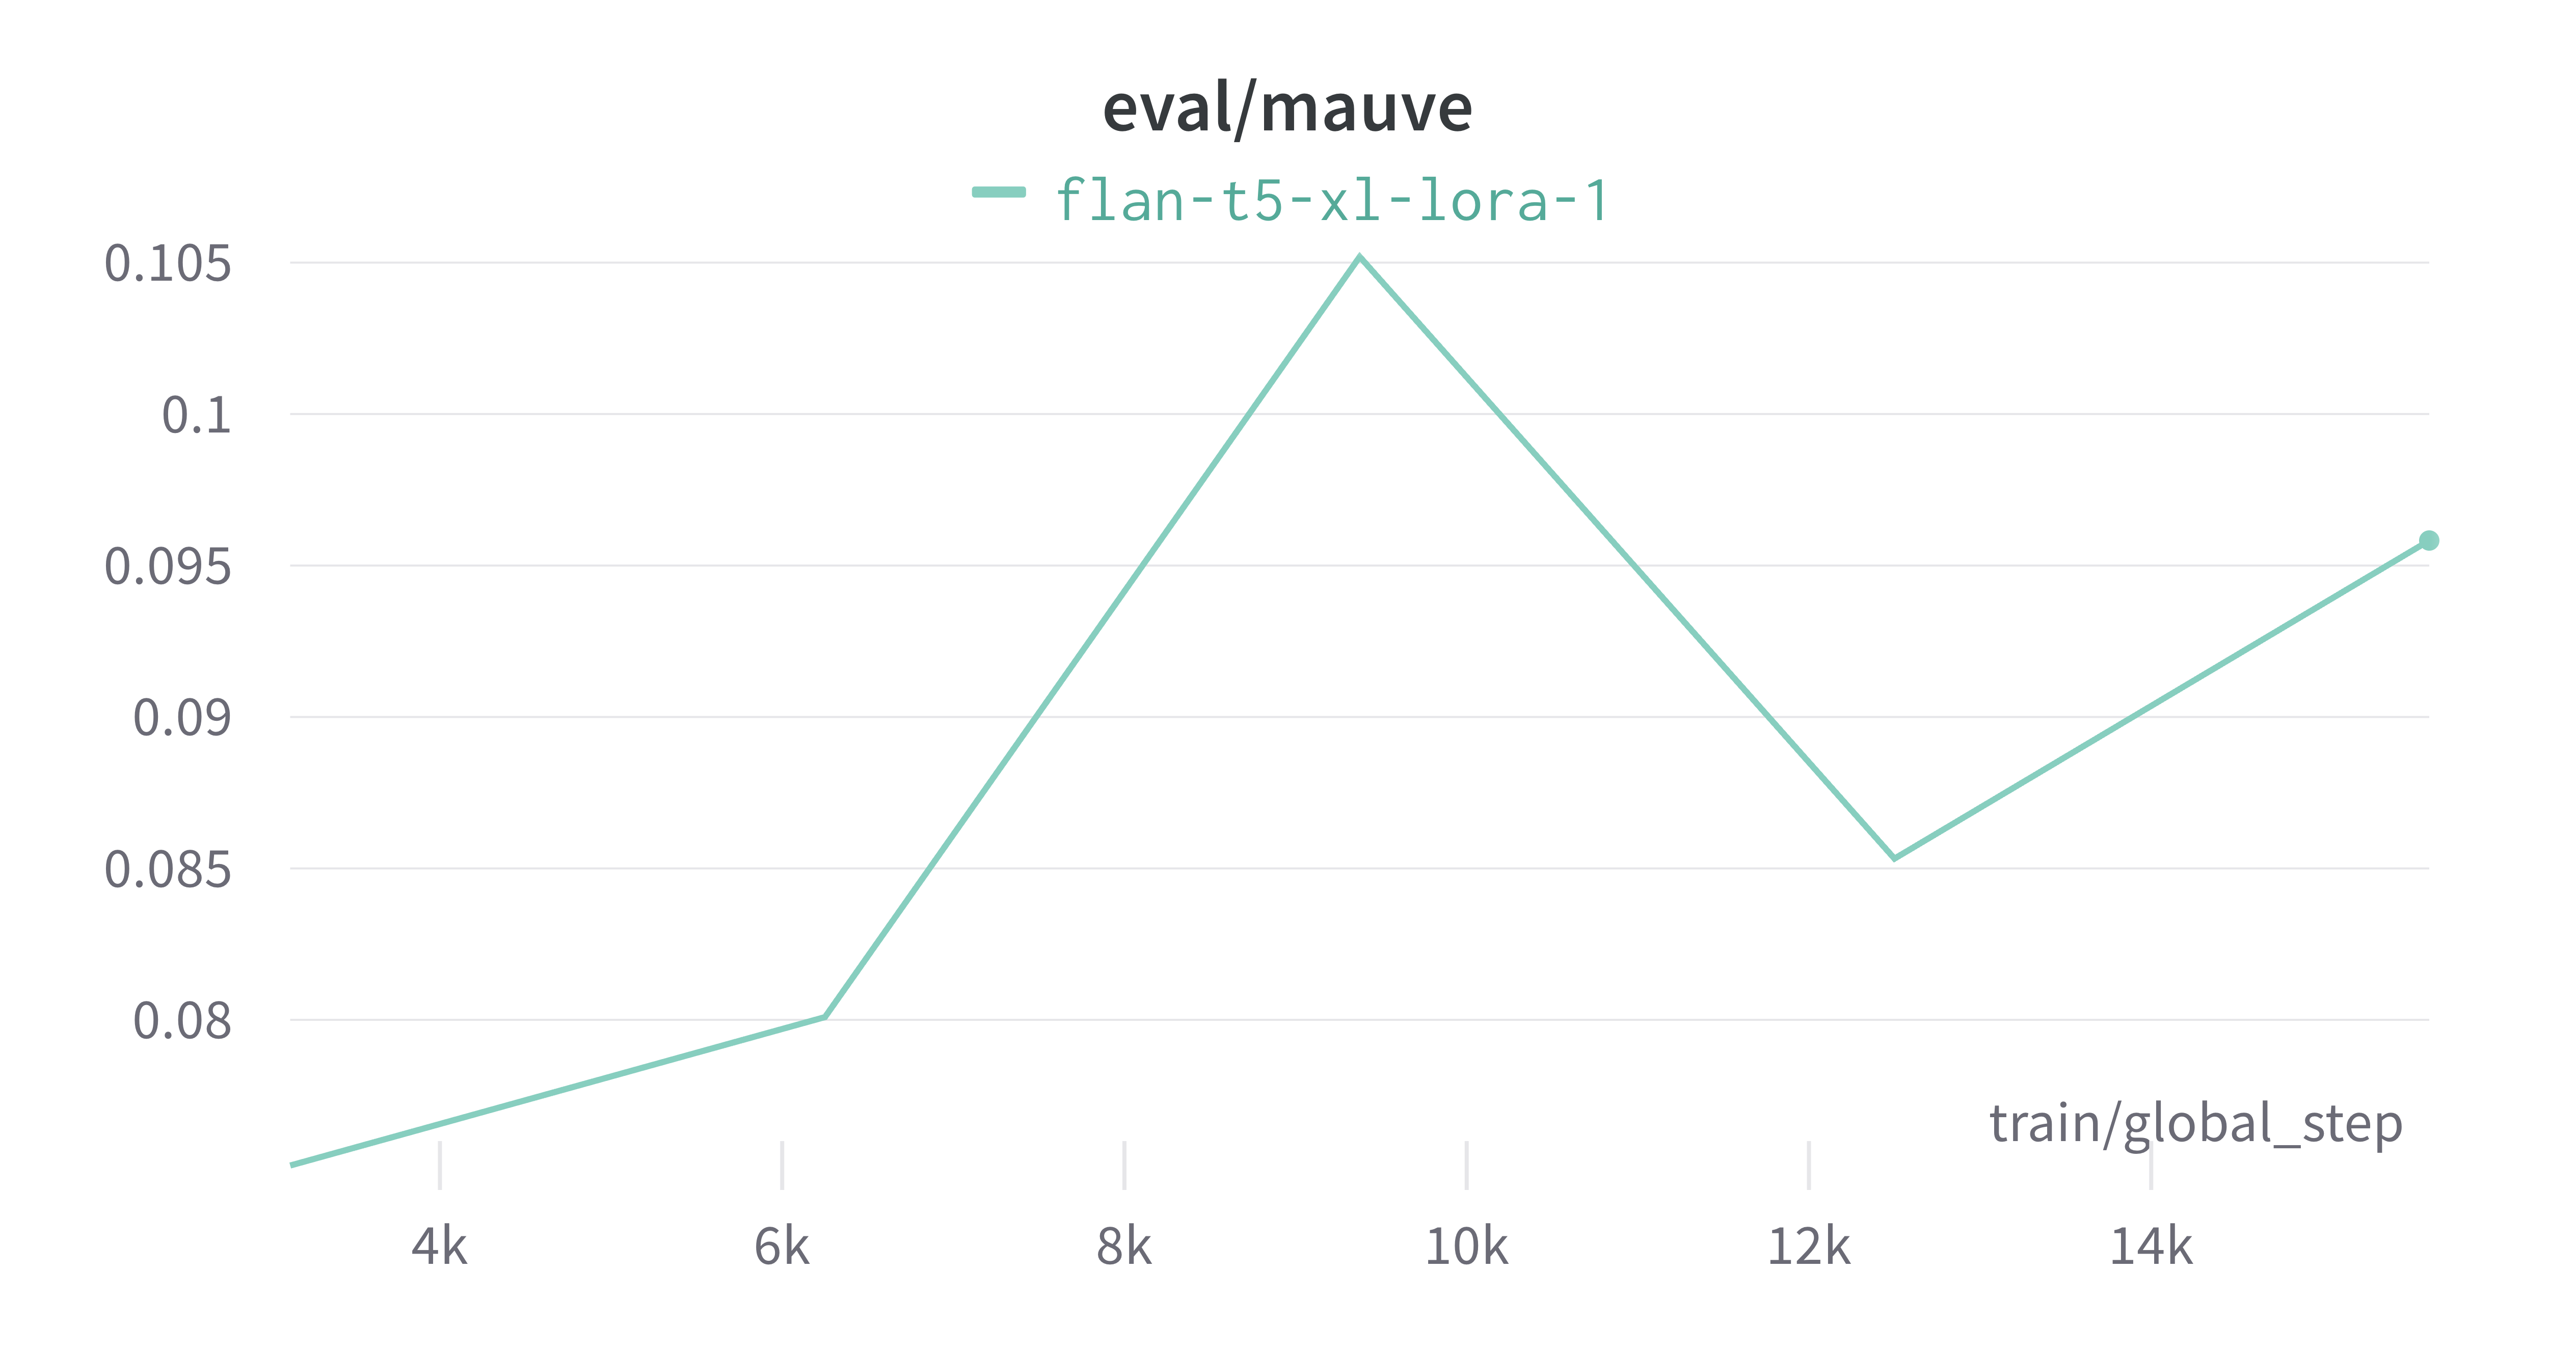
\includegraphics[width=.6\textwidth]{total-mauve}
  \caption{Значение метрики MAUVE на валидационных данных}
  \label{total-mauve}
\end{figure}


\addchap{ЗАКЛЮЧЕНИЕ}
В рамках данного исследования была поставлена цель разработки эффективной диалоговой модели, способной генерировать качественные ответы на основе образа неигрового персонажа и контекста диалога в игровой индустрии. Был использован специально созданный для исследования датасет DNDD (Dungeon \& Dragons Dialogues). И подготовлен специально для эмулирования диалогов в играх. В процессе экспериментов были рассмотрены различные параметры и планировщики скорости обучения.

На основе проведенных экспериментов можно сделать вывод о наилучшем выборе параметров для обучения модели. Для модели Flan-T5 Был выявлен оптимальный планировщик скорости обучения - константный планировщик, а оптимальное значение скорости обучения составляет $9 \times 10^{-4}$. Это сочетание показало лучшие результаты по функциям ошибок и метрикам на представленных наборах данных.

Однако, следует отметить, что введенная сложность задачи диалоговой моделирования в игровой индустрии, где ответы зависят от различных условий и контекста диалога, может быть причиной низких значений метрик Exact Match и MAUVE. Оценка Exact Match грубо оценивает результат генерации, причем даже переформулировка фразы может привести к низким значениям.

В целом, полученные результаты демонстрируют возможность обучения эффективной диалоговой модели на доступных вычислительных ресурсах. Однако, дальнейшие исследования и улучшения в области диалоговых моделей могут привести к более точным и качественным результатам.
\break

\begin{thebibliography}{99}
  \addcontentsline{toc}{chapter}{СПИСОК ЛИТЕРАТУРЫ}
  \bibitem{human-wer}
  Lippmann R. P. Speech recognition by machines and humans [Текст] // Speech communication. – 1997. – Т. 22. – №. 1. – С. 1-15.
  \bibitem{whisper}
  Radford A. et al. Robust speech recognition via large-scale weak supervision [Текст] // arXiv preprint arXiv:2212.04356. – 2022.
  \bibitem{state-of-gpt}
  Karpathy A. State of GPT [Электронный ресурс]. --- URL: \url{https://karpathy.ai/stateofgpt.pdf} (дата обр. 11.06.2023)
  \bibitem{transformer-paper}
  Vaswani A. et al. Attention is all you need [Текст] // Advances in neural information processing systems. – 2017. – Т. 30.
  \bibitem{backprop-theory}
  Hecht-Nielsen R. Theory of the backpropagation neural network [Текст] // Neural networks for perception. – Academic Press, 1992. – С. 65-93.
  \bibitem{optimizers-paper}
  Ruder S. An overview of gradient descent optimization algorithms [Текст] // arXiv preprint arXiv:1609.04747. – 2016.
  \bibitem{adafactor-paper}
  Shazeer N., Stern M. Adafactor: Adaptive learning rates with sublinear memory cost [Текст] // International Conference on Machine Learning. – PMLR, 2018. – С. 4596-4604.
  \bibitem{word2vec-paper}
  Mikolov T. et al. Efficient estimation of word representations in vector space [Текст] // arXiv preprint arXiv:1301.3781. – 2013.
  \bibitem{bpe-paper}
  Sennrich R., Haddow B., Birch A. Neural machine translation of rare words with subword units [Текст] // arXiv preprint arXiv:1508.07909. – 2015.
  \bibitem{gpt-paper}
  Radford A. et al. Improving language understanding by generative pre-training. – 2018.
  \bibitem{t5-paper}
  Raffel C. et al. Exploring the limits of transfer learning with a unified text-to-text transformer [Текст] // The Journal of Machine Learning Research. – 2020. – Т. 21. – №. 1. – С. 5485-5551.
  \bibitem{bert-paper}
  Devlin J. et al. Bert: Pre-training of deep bidirectional transformers for language understanding [Текст] // arXiv preprint arXiv:1810.04805. – 2018.
  \bibitem{sentencepiece-paper}
  Kudo T., Richardson J. Sentencepiece: A simple and language independent subword tokenizer and detokenizer for neural text processing [Текст] // arXiv preprint arXiv:1808.06226. – 2018.
  \bibitem{flan-paper}
  Chung H. W. et al. Scaling instruction-finetuned language models [Текст] // arXiv preprint arXiv:2210.11416. – 2022.
  \bibitem{weidu-repo}
  Репозиторий проекта WeiDU [Электронный ресурс]. --- URL: \url{https://github.com/WeiDUorg/weidu}
  \bibitem{llama-paper}
  Touvron H. et al. Llama: Open and efficient foundation language models [Текст] // arXiv preprint arXiv:2302.13971. – 2023.
  \bibitem{alpaca-docs}
  Документация Alpaca [Электронный ресурс]. --- URL: \url{https://crfm.stanford.edu/2023/03/13/alpaca.html} (дата обр. 06.06.2023)
  \bibitem{chatgpt-docs}
  Документация ChatGPT [Электронный ресурс]. --- URL: \url{https://openai.com/blog/chatgpt} (дата обр. 06.06.2023)
  \bibitem{MMLU-bench}
  Соревнование на наборе данных MMLU [Электронный ресурс]. --- URL: \url{https://paperswithcode.com/sota/multi-task-language-understanding-on-mmlu} (дата обр. 06.06.2023)
\end{thebibliography}

\appendix
\renewcommand{\thechapter}{\Asbuk{chapter}}
\chapter{ИСХОДНЫЙ КОД ОБРАБОТКИ DNDD}
\label{app:code}\texttt{\lstinputlisting[language={Python}, caption=$\text{Файл prepare.py}$]{./code/prepare.py}}
\texttt{\lstinputlisting[language={Python}, caption=$\text{Файл arg\_parser.py}$]{./code/arg_parser.py}}
\texttt{\lstinputlisting[language={Python}, caption=$\text{Файл descriptions.py}$]{./code/descriptions.py}}
\texttt{\lstinputlisting[language={Python}, caption=$\text{Файл dialogue\_data.py}$]{./code/dialogue_data.py}}
\texttt{\lstinputlisting[language={Python}, caption=$\text{Файл utils.py}$]{./code/utils.py}}

\chapter{ПРИМЕР ДИАЛОГА}
\label{app:diagogue}\texttt{\lstinputlisting[language={}, caption=$\text{Пример диалога}$]{./code/diagogue.txt}}

\end{document}
